\newlength\cmsTabSkip\setlength{\cmsTabSkip}{1ex}
\providecommand{\NA}{\ensuremath{\text{---}}}
\providecommand{\DOI}[1]{\href{http://dx.doi.org/#1}{\doi{#1}}}
\newcommand{\TENSORFLOW} {{\textsc{TensorFlow}}\xspace}
\newcommand{\PYTORCHGEOMETRIC} {{\textsc{PyTorch-Geometric}}\xspace}
\newcommand{\PYTORCH} {{\textsc{PyTorch}}\xspace}
\newcommand{\ONNX} {{\textsc{ONNX}}\xspace}
\newcommand{\ONNXRUNTIME} {{\textsc{ONNX Runtime}}\xspace}
\newcommand{\XGBOOST} {{\textsc{XGBoost}}\xspace}
%\usepackage{enumitem}


\cmsNoteHeader{ML-23-YYY}

\title{Portable Acceleration of CMS Mini-AOD Production with Coprocessors as a Service}

\address[cern]{CERN}
\author[cern]{The CMS Collaboration}

\date{\today}

\abstract{Computing demands for large scientific experiments, such as the CMS experiment at CERN, will increase dramatically in the next decades. To complement the future performance increases of software running on CPUs, explorations of coprocessor usage in data processing hold great potential and interest. We explore the novel approach of Services for Optimized Network Inference on Coprocessors (SONIC), and study the deployment of this as-a-service approach in large-scale data processing. In this setup, the main CMS Mini-AOD data processing workflow is executed on CPUs, while several machine learning (ML) inference tasks are offloaded onto (remote) coprocessors, such as GPUs. With experiments performed at Google Cloud, the Purdue Tier-2 computing center, and combinations of the two, we demonstrate the acceleration of these ML algorithms individually on coprocessors and the corresponding throughput improvement for the entire workflow. We also present that this approach can be easily generalized to different types of coprocessors, and even deployed on local CPUs without performance decrease. We emphasize that SONIC enables high coprocessor usage and brings the portability to run workflows on different types of coprocessors.
}

\hypersetup{%
pdfauthor={SONIC Team},%
pdftitle={Portable Acceleration of CMS Mini-AOD Production with Coprocessors as a Service},%
pdfsubject={CMS},%
pdfkeywords={CMS, Computing, Machine Learning}}

\maketitle

\section{Introduction}
\label{sec:intro}
During the first two runs of the CERN Large Hadron Collider (LHC)~\cite{Evans:2008zzb}, experimental collaborations, such as the ATLAS~\cite{ATLAS:2008xda} and CMS~\cite{CMS:2008xjf} collaborations, have analyzed trillions of high energy proton-proton collisions and produced an extensive suite of physics results. Among these are the discovery of the Higgs boson~\cite{ATLAS:2012yve,CMS:2012qbp} in the standard model (SM),  and world-leading constraints on various beyond the SM (BSM) physics scenarios, such as supersymmetry~\cite{ATLAS:2021hza, ATLAS:2021twp, ATLAS:2021kxv, CMS:2020fia, CMS:2021edw, CMS:2022vpy} and exotic heavy-particle or dark matter candidate productions~\cite{ATLAS:2022ozf, ATLAS:2021wob, CMS:2022usq, CMS:2022qej}. In order to pursue further SM measurements and BSM searches, the amount of LHC data and the associated data processing rates of the experiments are expected to increase dramatically in ongoing and future physics runs~\cite{Bruning:2015dfu}.

The high data-taking rates of ATLAS and CMS, which are currently in the range of 0.1--1\unit{PB/s} and planned to increase to $\mathcal{O}(10)\unit{PB/s}$, present a significant computational challenge for physicists to process the data~\cite{Zabi:2020gjd,2137107}. 
%Because it is neither feasible nor desirable to store such large volumes of data, both experiments employ two-level trigger systems to reduce the final rate to about 10\unit{GB/s}~\cite{ATLAS:2020esi, CMS:2016ngn}, often referred to as ``online''. After raw data is stored, it is processed to extract high-level information that is useful for analysis, referred to as ``offline''. 
A two-level trigger system is employed to run fast algorithms and reduce the data rate to about 10\unit{GB/s}~\cite{ATLAS:2020esi, CMS:2016ngn}; while this is a significantly smaller rate, it is still very challenging for subsequent processing steps. As shown in Fig.~\ref{fig:CPU_needs}, even with aggressive computing research and development and favorable budget increases, the projected computing needs for CMS will be only narrowly satisfied.

\begin{figure}[htp]
    \centering
    %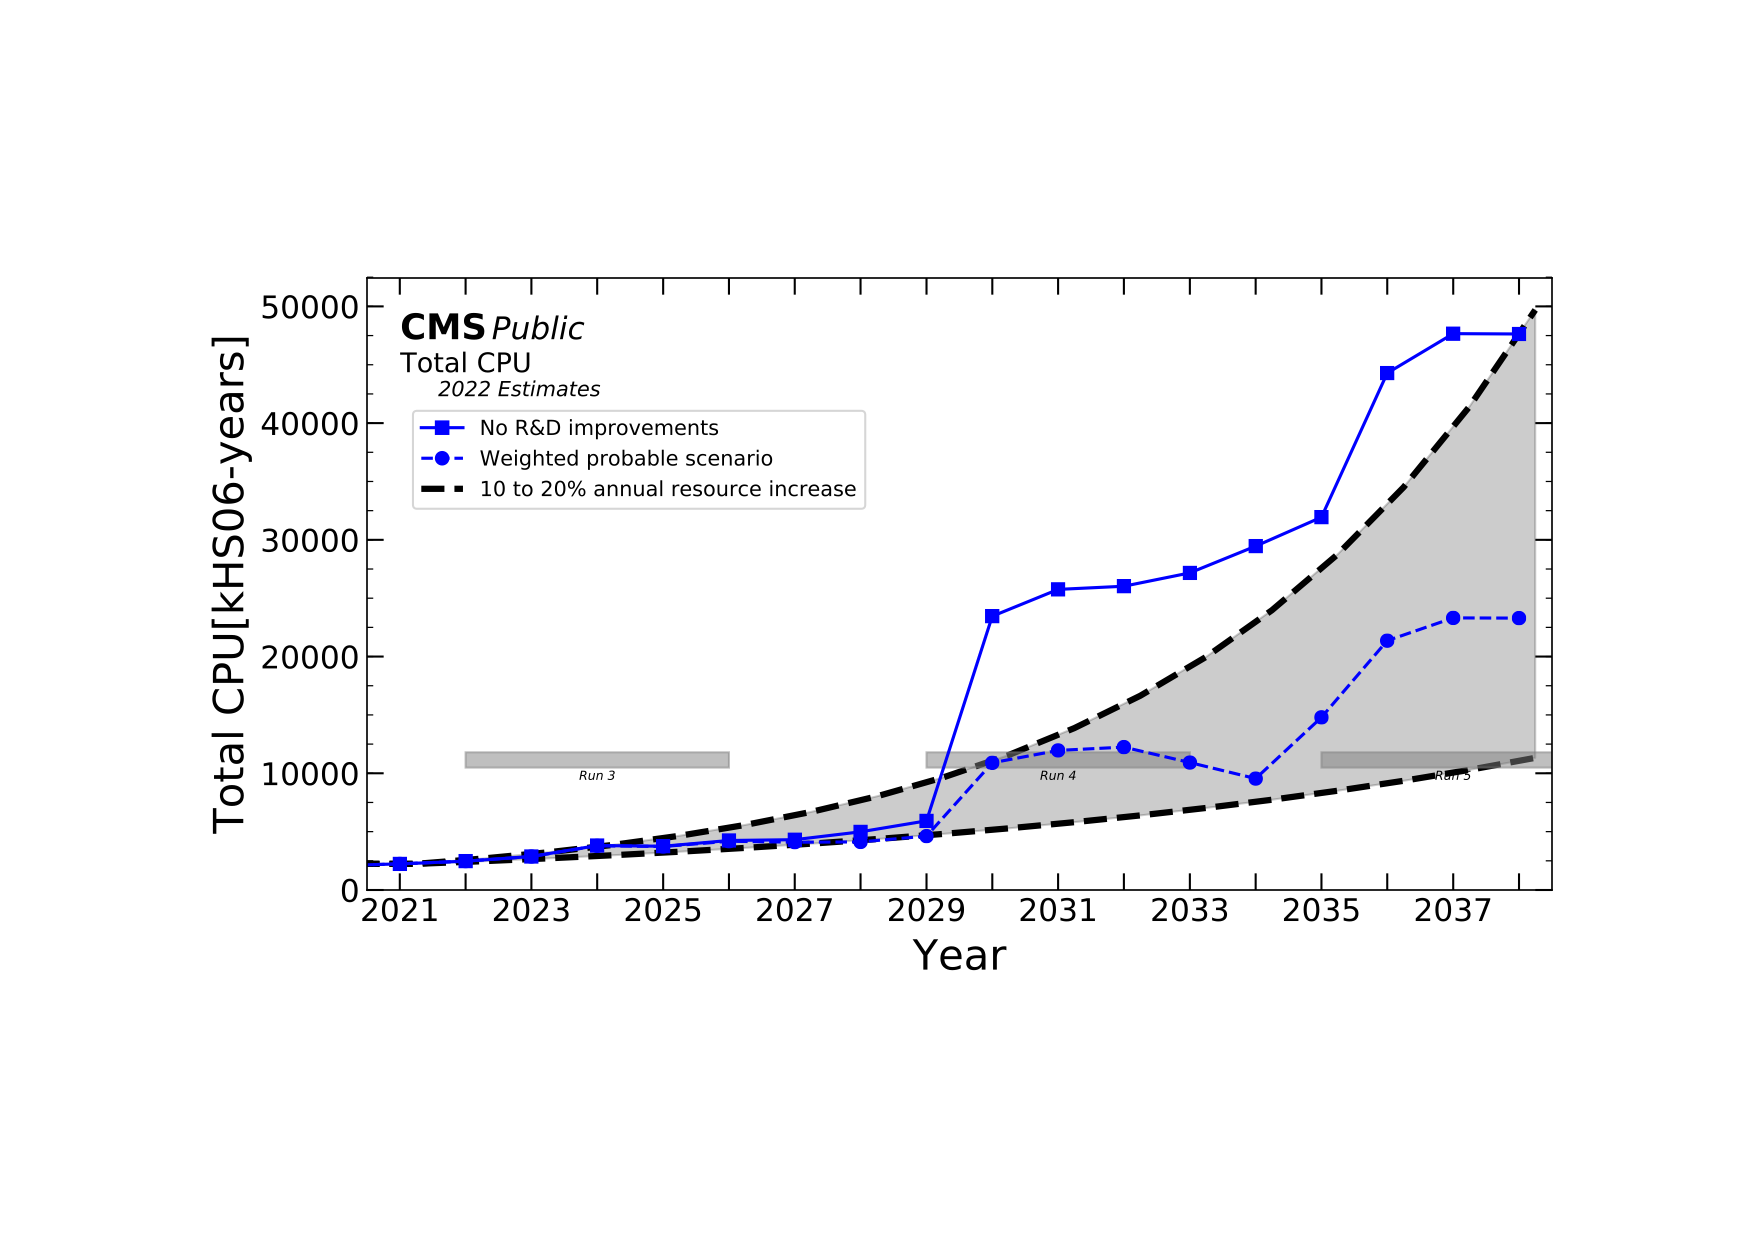
\includegraphics[height=7cm,trim={1cm 4cm 0 4cm},clip]{plots/cpu_cms2022.pdf}
    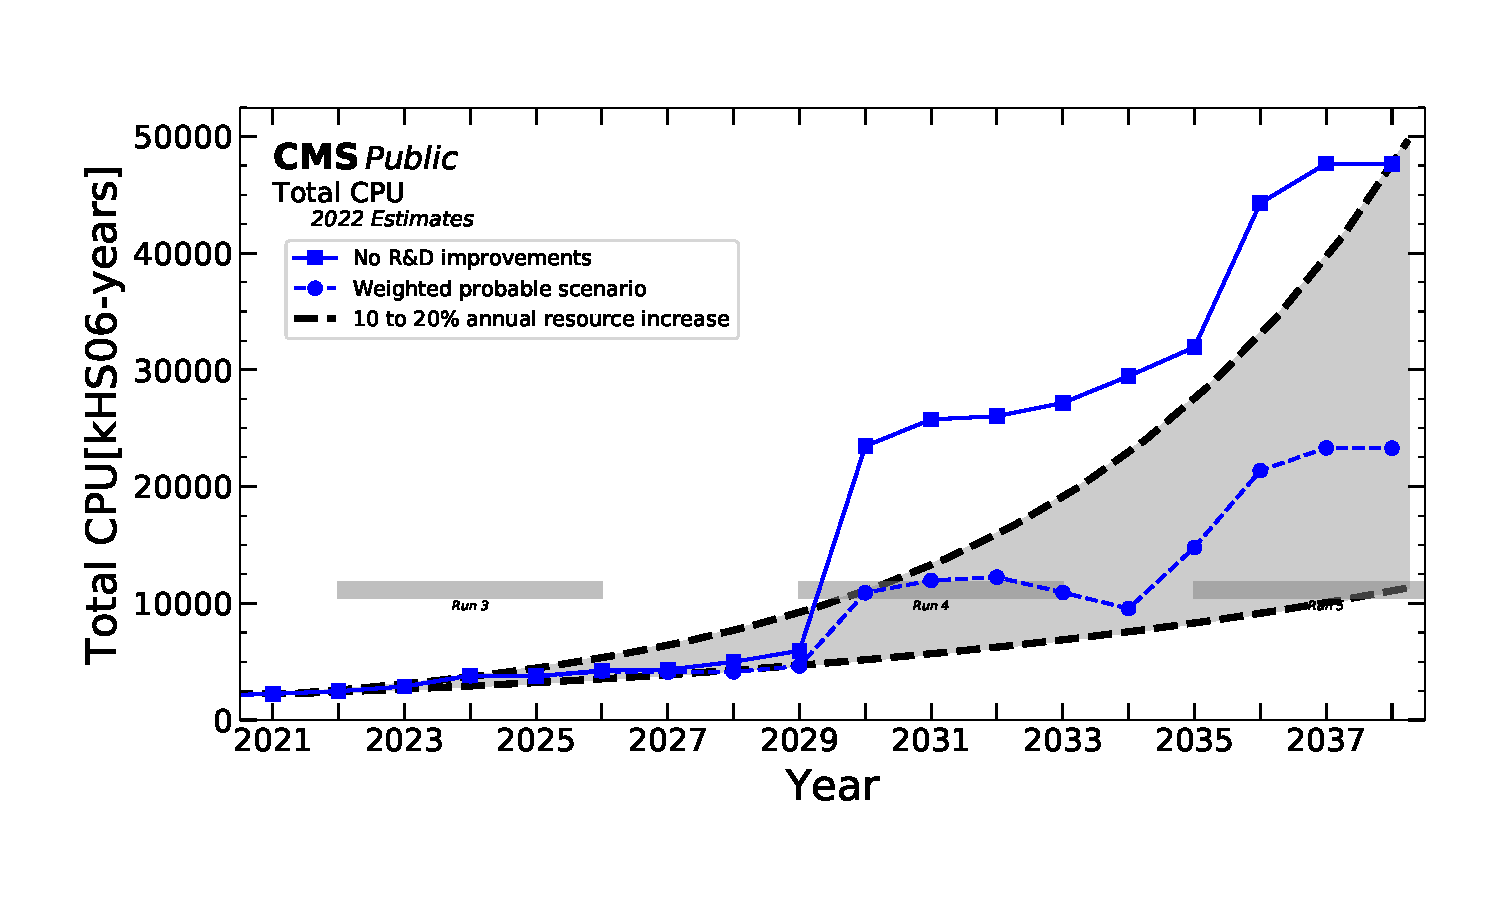
\includegraphics[height=7cm,trim={0 1cm 0 1cm},clip]{plots/cpu_cms2022_vectorized.pdf}
    %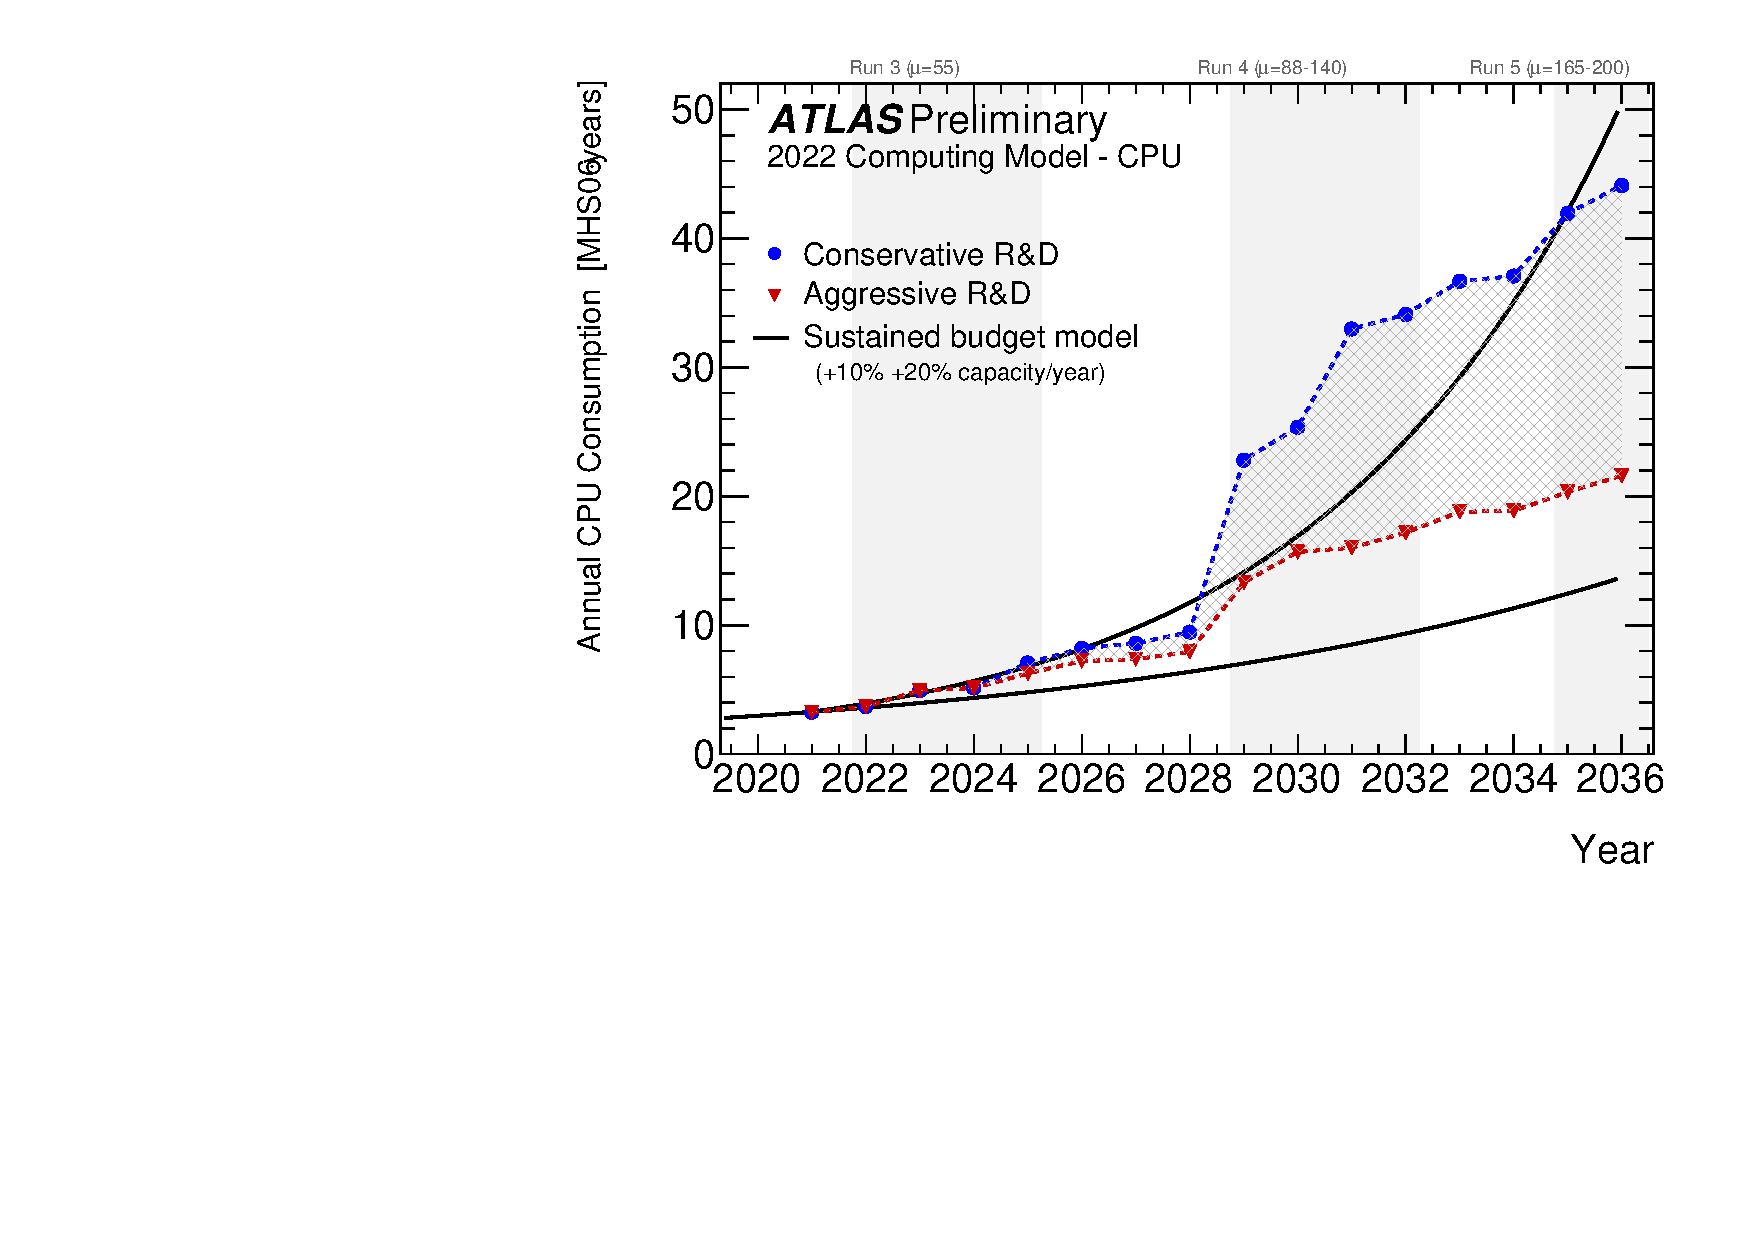
\includegraphics[width=0.75\textwidth]{plots/cpu_atlas2022.pdf}
    \caption{CPU time requirement projections for CMS offline processing and analysis needs~\cite{CMS_computing_plot, CMS:2815292}. Plot shows projected resource availability based on 10\% and 20\% annual budget increases. Lines are included for projections based on current performance and performance with expected research and development improvements. An analogous plot from ATLAS can also be found in Ref.~\cite{ATLAS_computing_plot}. }
    \label{fig:CPU_needs}
\end{figure}

\begin{sloppypar}While the expected performance increase of CPUs is limited, data processing can also be carried with a variety of modern architectures, such as graphics processing units (GPUs), field-programmable gate arrays (FPGAs), and application-specific integrated circuits (ASICs), which can collectively be referred to as ``coprocessors.'' These architectures are becoming increasingly popular because of their large numbers of processing units and inherent parallelization designs, especially suited for machine learning (ML) algorithm computations.\end{sloppypar} 
%Previous studies have shown that running ML algorithm inference on coprocessors can dramatically reduce the computation latency and increase the throughput for high energy physics (HEP) data processing~\cite{Duarte:2019fta, Krupa:2020bwg, Wang:2020fjr}. In addition, it is also possible to design domain algorithms that are specifically optimized for coprocessor acceleration, such as ``Patatrack,'' which is designed to run in a heterogeneous architecture in the CMS high-level trigger (HLT) system, reducing the per-event latency of the trigger~\cite{Bocci:2020pmi}.\end{sloppypar}

Within high energy physics (HEP), deep learning (DL) algorithms are already widely used for regression and classification tasks, and their popularity is growing rapidly~\cite{Guest:2018yhq, Albertsson:2018maf, Bourilkov:2019yoi, Larkoski:2017jix}. These algorithms can be easily accelerated on heterogeneous architectures and are taking up increasing fractions of the overall processing loads. For example, ML inferences takes about 10\% of the total processing time in one of the CMS data processing stages explained later. Therefore, developing a framework to enable and optimize the deployment and portability for coprocessors is of considerable interest to HEP experiments.

The most straightforward framework for deployment is to simply equip every CPU machine with coprocessors, referred to as ``directly-connected.'' In this scenario, every CPU thread within the machine can communicate with the coprocessor. However, since communications are limited to the CPUs and coprocessors within the same machine, it is hard to explore additional or different types of coprocessor resources. Besides, since the CPU-coprocessor ratio needs to be predetermined and fixed after deployment, the coprocessor resources are unlikely to be optimally utilized, leading to either wasted cost when under-saturating, or performance drops when over-saturating.

An alternative framework is ``inference as a service'' (IaaS), where coprocessor resources are factorized out of CPU machines. As represented in Fig.~\ref{fig:illustration}, in this scheme CPU-based \emph{clients} can send the computing request with necessary information to coprocessor-based \emph{servers} via network calls; servers running on coprocessor resources can perform computing tasks upon request. This removes the restriction of a coprocessor only being used by the CPUs directly connected to it, allowing it to accept processing requests from any CPUs (local or remote) as long as network communications are guaranteed. Certain types of coprocessors can be allocated for specific tasks, and the CPU-coprocessor ratio is flexible and dynamic. Resource utilization can therefore be optimized based on specific tasks, as the number of client-side jobs using a single server can be varied depending on the computational demands of a given task. Furthermore, at the software level, since the supports for coprocessors and CPU workflows are separated, it is easier to support different types of coprocessors. This ensures algorithm portability with minimal development or maintenance burden. The implementation of IaaS in experimental software frameworks can be accomplished using the Services for Optimized Network Inference on Coprocessors (SONIC) approach~\cite{Duarte:2019fta}.

\begin{figure}[htp]
    \centering
    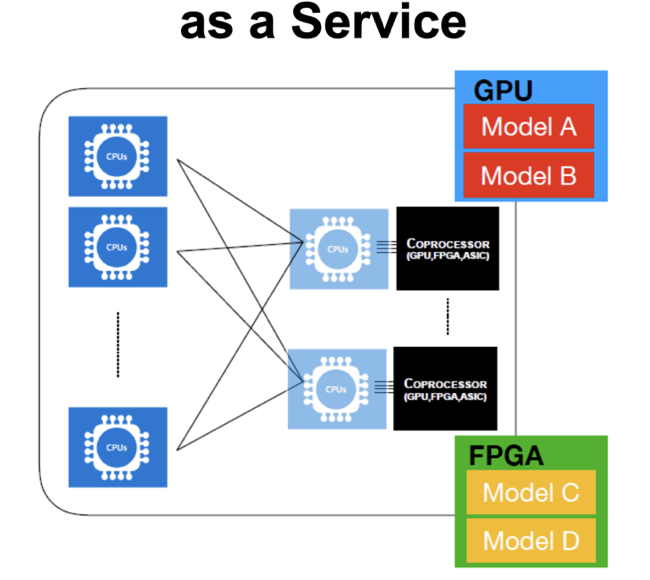
\includegraphics[width=0.50\textwidth]{plots/illustration.png}
    \caption{An illustration of an example inference as-a-service setup with multiple coprocessor servers. (\textcolor{red}{Plot to be updated: Jen suggested to include the directly-connected case for comparison. Otherwise remove ``as a Service" in the plot.})}
    \label{fig:illustration}
\end{figure}


SONIC has previously been demonstrated for CMS using GPUs with a variety of ML algorithms~\cite{Krupa:2020bwg}, showing offloading ML algorithms with SONIC bringing little extra computation latency and a corresponding increase in the throughput.
The approach has also been used in other experiments, including protoDUNE~\cite{Wang:2020fjr}. There, a 2.7 times reduction in the total processing time per event compared to a CPU-only architecture was achieved.

Heterogeneous computing frameworks using GPUs have appeared in multiple non-IaaS contexts in HEP recently as well. One of the first significant real-time applications was in the ALICE high-level trigger system~\cite{ALICE:2018phe}, where GPUs were used to accelerate online tracking. Similarly, a fully GPU-based implementation of the first level trigger has been implemented for LHCb~\cite{Aaij:2019zbu}, which could be run on about 500 GPUs. In CMS, a GPU-specific version of the pixel tracking domain algorithm called ``Patatrack'' was developed, along with several other local reconstruction algorithms, which are now employed in the high-level trigger for Run 3 to reduce the per-event latency~\cite{Bocci:2020pmi}. For a further overview of GPU usage in real-time applications for HEP, please see Ref.~\cite{VomBruch:2020plx}.

In this paper, we take the Mini-AOD data~\cite{Petrucciani:2015gjw} production workflow as an example, and study the deployment and the performance gains of the IaaS framework. In the current Mini-AOD production workflow, about 10\% of the computing time is consumed by ML algorithm inferences, which can be easily accelerated on GPUs. We firstly summarize studies of the optimization and acceleration of the inference of each individual ML algorithm on GPUs. Then we show that the IaaS scheme, which is implemented in the CMS software framework \CMSSW~\cite{CMS:2006myw} via SONIC, not only decreases processing latency but can also be deployed in large-scale production to optimize GPU utilization. Finally, we show that the SONIC approach can be easily ported to different types of coprocessors, and run as well on local CPUs without performance decrease.

The paper is organized as follows. Section~\ref{sec:cmscomputing} provides a brief overview of the CMS computing architecture, and the Mini-AOD data production workflow. Section~\ref{sec:sonic} discusses in detail SONIC, including the technical implementation in \CMSSW, the current inference servers, and the SONIC features. Section~\ref{sec:algo} includes the dataset used for the studies and the algorithms ported to SONIC.
Section~\ref{sec:performances} provides the algorithm inference optimizations and performance results from the tests. Portability to different types of processors, including local CPUs and Graphcore Intelligence Processing Units (IPUs)~\cite{Graphcore, IPU_Perf} coprocessors is presented in Section~\ref{sec:IPUs}. Finally, Section~\ref{sec:summary} summarize the studies and discusses future plans.

\section{The CMS Computing Model}
\label{sec:cmscomputing}
This section describes the computing setup of the CMS experiment, the software framework \CMSSW, and the Mini-AOD data production workflow.

\subsection{Introduction to CMS Computing}
\label{sec:implementation}

The LHC provides countercirculating beams of high energy protons, such that bunches of protons in these beams can interact with each other in the center of the CMS detector~\cite{CMS:2008xjf} every 25\unit{ns}. When protons from the countercirculating beams collide, a large variety of physical processes can occur, which then lead to the creation of either fundamental or composite particles. These particles, or their decay products, can then propagate into the CMS detector, which is designed to determine the type, energy, and momentum of each particle. Each bunch crossing where proton collisions occurs is referred to as an ``event'', in which hundreds of particles can be projected into the CMS detector. The detector itself comprises multiple layers including silicon pixels and strips, crystal calorimeters, sampling calorimeters, and muon spectrometers. Each component of the detector has active components that create electrical signals when particles interact with them, either from their charge or through interactions with the material's atomic electrons or nucleus. Each discrete signal can be called a hit.

\subsection{\CMSSW}
\label{sec:cmssw}
One purpose of the \CMSSW software stack is to extract high-level physics information for each event from these hits. In essence, physicists can use \CMSSW to determine which of the large number of possible physical processes occurred in a given event, be it something relatively rare, such as the creation of a Higgs boson, or something as common the scattering of gluons in colliding protons. CMSSW processes each event with a sequence of algorithms, converting hits from electrical signals to positional and energy measurements, linking these measurements into clusters~\cite{CMS:2020uim} and trajectories~\cite{CMS:2014pgm}, combining trajectories and clusters into single particle representations and jets corresponding to hadronic showers~\cite{CMS:2017yfk}. Additional algorithms in CMS can be run to determine quantities such as the total imbalance of energy across the axis defined by the proton beam line or tag jets as containing or being produced by rare particles.

The \CMSSW framework uses Intel Threading Building Blocks~\cite{tbb} to enable task-based multithreading. As explained in Ref.~\cite{Bocci:2020olh}, this multithreading implementation allows for asynchronous non-blocking calls to external resources, such as a GPU, via ``ExternalWork''. This setup optimizes CPU resource utilization by minimizing downtime; the CPU is allowed to continue executing algorithms that do not require a coprocessor or depend on the results of the coprocessor-dependent algorithm while waiting for the external call to return.

\subsection{Mini-AOD production}
\label{sec:miniaod_production}
CMSSW is used both in online and offline contexts within CMS. While the Level-1 trigger is hardware-based, the high-level trigger (HLT) is constructed from algorithms in CMSSW. CMSSW also contains the algorithms that are used to process the raw data after it has been stored, deriving the higher-level information useful to physicists. The centralized offline CMS data processing flow involves a few steps. The first creates an ``analysis object data'' (AOD) format derivation of every raw event. Then the second creates a slimmed, higher-level ``Mini-AOD''derivation~\cite{Petrucciani:2015gjw}. Finally the third creates a further slimmed ``NANOAOD" format that contains only top-level information used for physics analyses~\cite{Rizzi:2019rsi}. Because algorithms within \CMSSW are occasionally modified, the raw data is reprocessed regularly. The AOD derivation step is performed on a yearly base and the subsequent Mini-AOD step is typically performed roughly a few times per year .

Mini-AOD files are designed to be relatively small and accessible, providing the high-level physics information needed for most analyses. They are derived from the AOD data format, reducing the size per event by a factor of 10. Mini-AOD processing involves a wide variety of algorithms that propagate, skim, and reanalyze the AOD input objects. 

\section{SONIC}
\label{sec:sonic}
This section describes the detailed implementation of SONIC in \CMSSW; the server used to serve models, NVIDIA Triton Inference Server; and the benefits of running inference with SONIC.

\subsection{Past Studies of SONIC}
\textcolor{red}{This section can probably be shortened and merged into the later section.}

The SONIC approach~\cite{SONIC_origin, SONIC_cms} was introduced in the first notable use of the IaaS scheme in HEP, which employed FPGA coprocessors to accelerate ML algorithms~\cite{Duarte:2019fta}. In this application, the ResNet-50 convolutional neural network~\cite{ResNet50} was retrained as a top quark jet tagger and as a neutrino event classifier. These algorithms were then hosted on the Microsoft Brainwave service~\cite{Brainwave}. It was shown that IaaS enabled per-inference latency reductions by a factor of more than 30, even including overhead and data transfer time between client jobs at Fermilab in Illinois and the Microsoft data center in Virginia.

This work was then extended to study the use of GPUs as coprocessors for multiple LHC-specific applications in Ref.~\cite{Krupa:2020bwg}. There, SONIC was used to enable acceleration of three algorithms:
\begin{enumerate}
    \item A ResNet-50 based top quark jet tagger;
    \item Fast Calorimeter Learning (FACILE), which is a deep neural network for CMS hadron calorimeter (HCAL) energy regression;
    \item DeepCalo, which is a convolutional neural network for electron and photon energy regression in the ATLAS electromagnetic calorimeter~\cite{deepcalo}.
\end{enumerate}
These algorithms represent a wide range of algorithmic complexity and input data size, and all of them show significant speed improvements when running via SONIC. While these algorithms provided an interesting and useful testbed, currently they are not run by default in either the ATLAS or CMS data-processing workflows.

The initial FPGA-based demonstration was similarly extended to a detailed study of GPU-based acceleration in the neutrino experiment context in Ref.~\cite{Wang:2020fjr}. There, the track and particle shower hit identification components of the ProtoDUNE-SP reconstruction chain~\cite{DUNE:2020cqd} were accelerated by a factor of 17. This lead to a 2.7 times reduction in the total processing time per event compared to a CPU-only architecture. In this application, a single GPU could be used to service 68 CPU threads, which is an important demonstration of the flexibility to optimize the CPU-coprocessor ratios in the IaaS paradigm.

Heterogeneous computing frameworks using GPUs have appeared in multiple non-IaaS contexts in HEP recently as well. One of the first significant real-time applications was in the ALICE high-level trigger system~\cite{ALICE:2018phe}, where GPUs were used to accelerate online tracking. Similarly, a fully GPU-based implementation of the first level trigger has been planned for LHCb~\cite{Aaij:2019zbu}, which could be run on about 500 GPUs. For a further overview of GPU usage in real-time applications for HEP, please see Ref.~\cite{VomBruch:2020plx}.

In the CMS context, an algorithm that could accelerate tracking on GPUs with a parallelized cellular automaton approach was introduced in Ref.~\cite{Funke:2014dga}. Using a GPU-enabled heterogeneous architecture in the first layer of the CMS trigger for track triggering was then proposed in Ref.~\cite{Pantaleo:2016ery}, and a GPU-specific version of tracking called ``Patatrack'' has been developed which allows more complex tracking to be performed in triggering stages of data analysis~\cite{Bocci:2020pmi}. The authors of this algorithm proposed a mechanism for \CMSSW jobs to directly interact with local co-processor resources~\cite{Bocci:2020olh}. Similarly, the use of GPU and FPGA resources was investigated to take advantage of the inherent parallelizability of local reconstruction algorithms for the CMS Electromagnetic and Hadronic calorimeters~\cite{Massironi_2020}.%and the use of GPU and FPGA resources was investigated to take advantage of the inherent parallelizability of local reconstruction algorithms for the CMS Electromagnetic and Hadronic calorimeters~\cite{Massironi_2020}. More recently, a GPU-specific version of tracking called ``Patatrack'' has been developed which allows more complex tracking to be performed in triggering stages of data analysis~\cite{Bocci:2020pmi}, and the authors of this algorithm proposed a mechanism for \CMSSW jobs to directly interact with local co-processor resources~\cite{Bocci:2020olh}.
%In neutrino physics, GPUs have been used to accelerate particle reconstruction tasks for IceCube~\cite{IceCube_tracking}.

\subsection{SONIC Implementation in \CMSSW}
SONIC is implemented in \CMSSW using the ExternalWork framework component, accessing coprocessor resources on remote servers via gRPC calls~\cite{gRPC}. An illustration of this procedure, where client jobs make asynchronous, non-blocking gRPC calls to a remote server, is shown in Fig.~\ref{fig:architecture}. An important aspect of this scheme is that the client-side code does not need to be able to run any particular inference packages or frameworks; it simply has to collect the relevant input data for a trained model, communicate that information to the server in the expected format, and handle the output from the server.

\begin{figure}[htp]
    \centering
    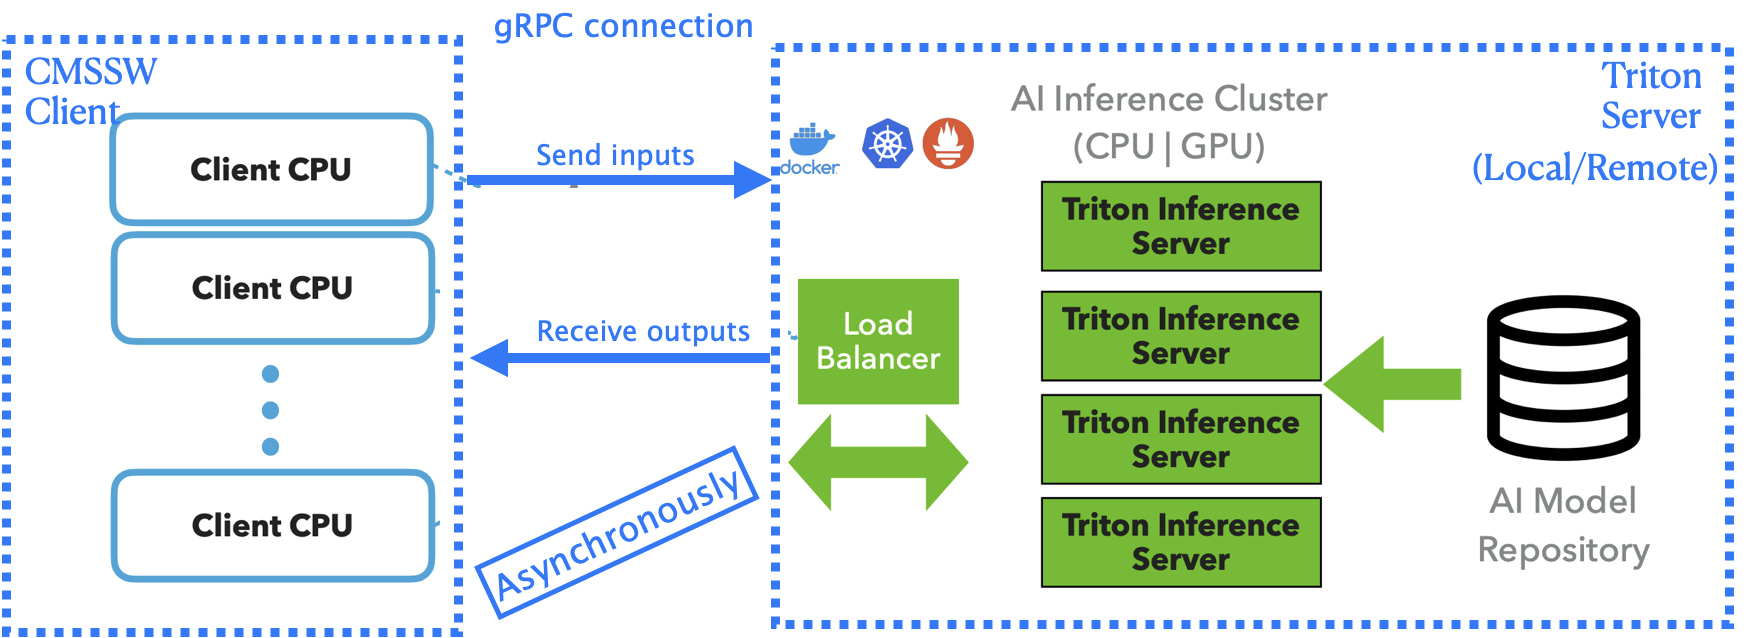
\includegraphics[width=0.90\textwidth]{plots/Architecture.png}
    \caption{Illustration of the SONIC implementation of inference as-a-service in \CMSSW. This figure also shows the possibility of an additional load-balancing layer in the SONIC scheme; for example, if multiple coprocessor-enabled machines are used to host servers, a Kubernetes engine can be set up to distribute inference calls across the machines. \textcolor{red}{(Plot will be updated to better quality)}}
    \label{fig:architecture}
\end{figure}

Within CMSSW, a mechanism has been implemented to account for the possibility that a client job cannot access a specified server for whatever reason. In this case, a ``fallback'' server is automatically created using either GPU resources if they are available or the CPU resources allocated to the client job in question. The client then makes gRPC calls to that local fallback server, which introduces negligible latency. The server overhead generally consumes very little of the CPU resources beyond what would be used for conventional inference, such that the per-event latency is not strongly affected by SONIC relative to running without SONIC. Fallback servers are automatically shut down when the job finishes. Studies related to these fallback servers are discussed in Section~\ref{sec:fallback}.

\subsection{NVIDIA Triton Inference Server}
\label{sec:triton}
%Document a brief introduction about the NVIDIA Triton inference server

As shown in Fig.~\ref{fig:architecture}, the GPU-based implementation of SONIC in \CMSSW uses the NVIDIA Triton Inference Server to deploy ML inference on the coprocessors~\cite{triton, triton_readme}. Triton servers can perform inference for ML algorithms, or ``models'', in most modern formats, including \PYTORCH, TensorRT, ONNX Runtime, \TENSORFLOW, and \XGBOOST, and also supports custom backends for alternative tasks. A single server can host multiple models at the same time or even multiple instances of the same model to allow concurrent inference requests. Triton also supports dynamic batching: if multiple inference calls are made within a window of time, the server can concatenate all calls' inputs into a single batch, which improves the GPU utilization and therefore increases the overall throughput. Parameters such as the number of model instances on a single server, the length of a batching window, and the optimal batch size are tunable and can be optimized on a case-by-case basis. Triton provides a model analyzer tool to aid in this optimization~\cite{triton_model_analyzer}.

Triton servers can use one or multiple GPUs on the same machine with a built-in load balancer. Triton servers can also run purely on CPU resources when there are no GPU resources available. For other types of coprocessors, Triton servers can also be used with the help of custom backends. To start a server, it is only necessary to provide a trained model file and sometimes a configuration file specifying input and output variable names, shapes, types, and model versions. Client-side jobs are configured with servers' address and port numbers in order to carry out communications, and jobs must provide input with the correct format for inference.

It is important to note that Triton provides an open source solution for implementing IaaS, with a public set of protocols. It is also possible to use those protocols in alternative server implementations, as was done in the FPGAs-as-a-Service Toolkit~\cite{FaaST}.%not strictly necessary to use Triton's set of protocols; for example, server protocols were independently reimplemented for communication with inference servers in the FPGAs-as-a-Service Toolkit~\cite{FaaST}.

\subsection{SONIC Discussions}
\label{sec:sonic_benefits}
\textcolor{red}{This section should also includes the discussions on the possible extra costs with SONIC: memory, network, complexity, and the compare the tradeoffs between SONIC and direct inferences.}

While many of the benefits of running with SONIC have been mentioned throughout the preceding text, it is worthwhile to quickly summarize some of these points here.
\begin{itemize}
    \item \emph{Containerization}: SONIC factorizes ML frameworks out of the client software stack, i.e., \CMSSW, making it easier support a wide variety of ML models. Currently, any ML algorithms in \CMSSW must either be cast in one of a limited number of supported frameworks, or else support for a new framework must be added. With SONIC, one can use any framework supported by Triton, including custom backends, with no modification of \CMSSW needed. This allows physicists to pick the best ML inference backend with less concern for the implementation details. This ``support'' for a wide variety of frameworks is easy to maintain.
    \item \emph{Simplicity}: Because of the containerization discussed above, client-side code that takes advantage of SONIC can be simplified. Generic functions for sending input to and receiving output from servers can be defined, and then to deploy any model deployed in the workflow, client code only needs to format model inputs correctly and collect the outputs.
    \item \emph{Flexibility}: In the SONIC paradigm, the ratio of CPU resources to GPU resources is not fixed, as clients from many different machines can access a single server running on either one GPU or multiple GPUs. Similarly, a single client can access multiple different servers running on multiple different machines. GPU-to-CPU ratios can therefore be adjusted for different ML inference tasks, allowing optimal utilization of coprocessor resources.
    \item \emph{Efficiency}: SONIC enables superior utilization of coprocessor resources. By optimizing the GPU-to-CPU ratio, it is easier to come close to saturating GPU resources without oversaturating them. Because of this, any GPU purchase can be kept to the minimal number of GPUs necessary, saving overall cost.
    \item \emph{Portability}: Through the use of SONIC, client-side workflows do not have to be modified to take advantage of different types of coprocessors. As long as a consistent protocol exists for communicating with the inference server, it does not matter if the server is on a CPU, GPU, FPGA, IPU, or any other architecture. This allows users to easily take advantage of whatever resources are available and easily optimize workflows if there are multiple options.
    \item \emph{Accessibility}: It is worth explicitly pointing out that SONIC is the only way for any CPU to access remote GPUs or other coprocessors. This should reduce costs associated with coprocessor-based inference acceleration, allowing for collaborators to share resources more easily. While calls to a remote server introduce a distance-dependent latency, the use of asynchronous calls in SONIC means that the overall event latency is negligibly impacted~\cite{Krupa:2020bwg}. SONIC can also use local resources if they are available.
\end{itemize}



\section{Physics Datasets and Algorithms}
\label{sec:algo}
%Document the algorithms we ported to SONIC, i.e., ParticleNet~\cite{Qu:2019gqs} + DeepTau~\cite{CMS:2022prd} + DeepMET. Include the algorithms and their implementations in CMSSW. Tables and PieChart about the latency breakdowns of these algorithms for Run-2 and Run-3. Discuss ragged batching? What about ECAL DRN? cite ECAL-specific note when released

%\textcolor{red}{Include IO sizes for these models. maybe also add them into Table~\ref{table:SONIC_Algos}}.

This section describes in detail the physics dataset, the ML algorithms ported to SONIC for inference, and the computing resources used in the studies.

\subsection{Dataset}
In the studies we chose to run on the Run-2 simulated $\ttbar$ dataset. They are copied to local disk to avoid remote I/O limitations for the benchmarks. Figure~\ref{fig:algorithms} shows that the per-event latency is about 993\unit{ms} when processing these \ttbar events on a 20-core Intel Haswell machine, when it is running five synchronized four-threaded jobs.

\begin{figure}[htp]
    \centering
    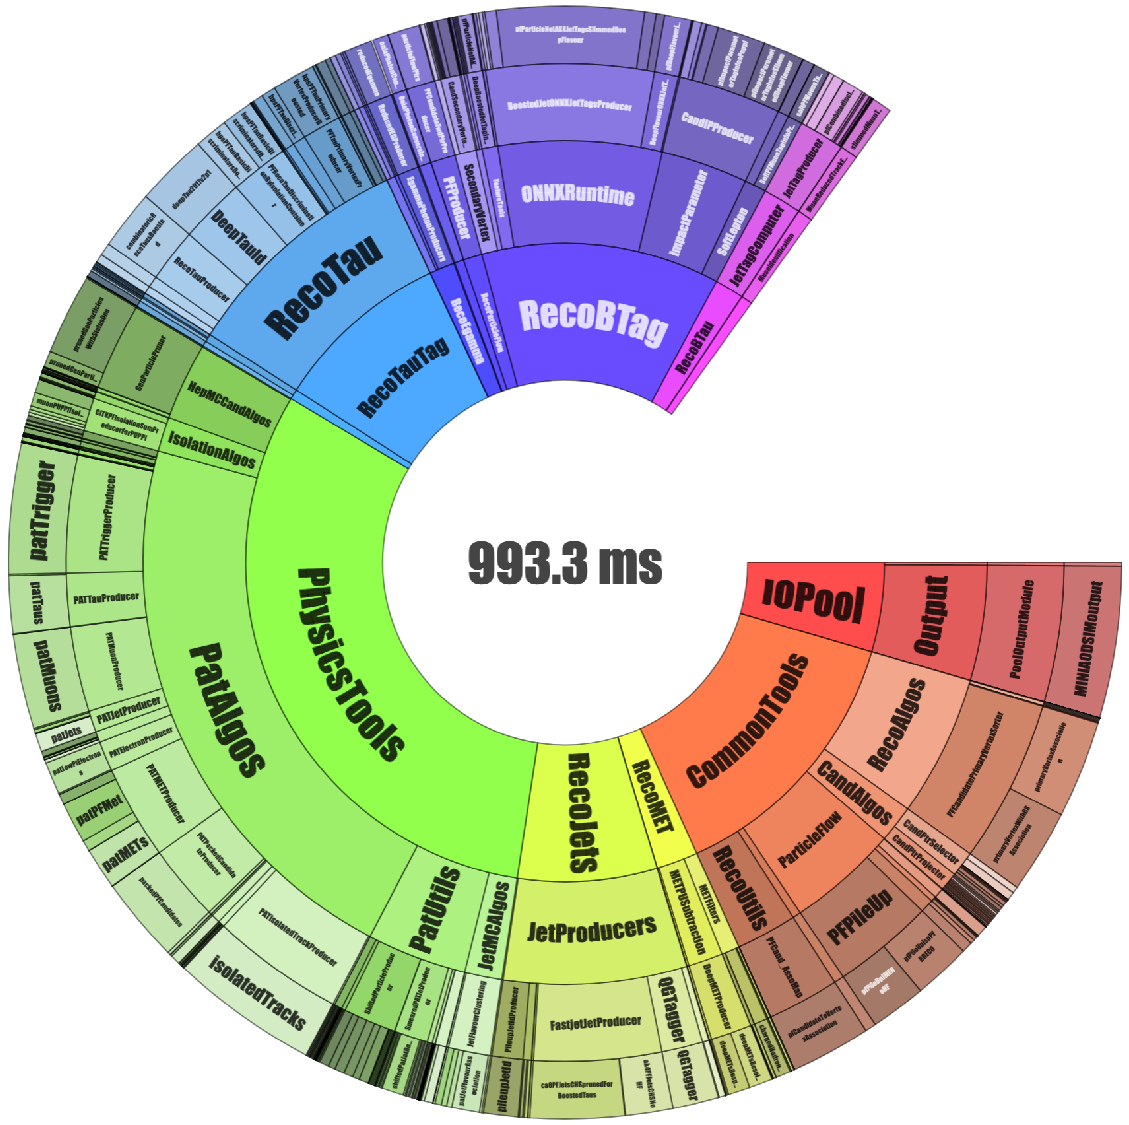
\includegraphics[width=0.50\textwidth]{plots/Step2_pieChart.pdf}
    \caption{Pie chart representing the per-event latency of various algorithms in a typical Mini-AOD processing for LHC Run 2 \ttbar events. \textcolor{red}{TODO: highlight the SONIC-ML part in the PieChart.}}
    \label{fig:algorithms}
\end{figure}


\subsection{Algorithms Ported to SONIC}

Adapting an ML algorithm to work within in SONIC requires a small effort to write code to prepare the network inputs and save the network outputs within CMSSW. In these studies, we tested three ML-based algorithms in the Mini-AOD workflow that are computing-intensive:

\subsubsection{ParticleNet}
\label{sec:PN}

ParticleNet (PN)~\cite{Qu:2019gqs} is a graph-neural-network-based algorithm for jet tagging and regression that represents jets as ``particle clouds''. Here, ``tagging'' refers to identifying jets as arising from specific particles. PN was trained in \PYTORCH~\cite{pytorch}, which is a framework not currently supported in \CMSSW, and exported to the \ONNX format~\cite{onnx}, which is supported in \CMSSW for fast inference. However, it is important to note that with SONIC, it is possible to perform inference with PN in the following formats: \ONNX; \PYTORCH; and \PYTORCH with TensorRT (TRT)~\cite{tensorRT}, which optimizes model performance on NVIDIA devices.

There are four different trained versions of PN currently running in the Mini-AOD workflow for different purposes:
\begin{enumerate}
    \item tagging anti-\kt jets~\cite{Cacciari:2008gp}, clustered with the \FASTJET package~\cite{Cacciari:2011ma}, with a radius of 0.4 (AK4 jets),
    \item tagging anti-\kt jets with a radius of 0.8 (AK8 jets)~\cite{Sirunyan:2020lcu},
    \item mass-decorrelated tagging for AK8 jets~\cite{Sirunyan:2020lcu}, and
    \item mass regression for AK8 jets~\cite{CMS-DP-2021-017}.
\end{enumerate}
All PN variations can be hosted on Triton servers.

The inputs to PN are the kinematic and flavor properties of the particle constituents of each jet and the secondary vertices associated with the jet. The inputs are permutation invariant, and information for up to 100 particles and 10 vertices is used; if there are more than 100 particles in a jet, the 100 particles with the highest \pt are used (for AK4 jets, the maximum numbers of particles and vertices are 50 and 5, respectively). For the three tagging versions of PN, the outputs of each inference are category probabilities for a variety of pre-defined jet categories, such as the presence of a Higgs boson or the presence of a top quark. For the mass regression, the output is a single value: the predicted jet mass.

In Mini-AOD processing, inference is performed separately for each jet in a given event, so the number of PN inferences depends on the specific physics processes and can vary substantially from event to event. When running the standard \CMSSW version of PN, no inference batching is performed, so each inference is truly performed separately. In this context, each inference can have a variable number of inputs with no padding involved. When using SONIC for PN, it is easiest to batch all of the jets in an event into a single inference request, such that input particle and secondary vertex information for each jet in an event is sent to the server in a single request. In subsequent performance studies, a ``maximally-padded'' approach is taken, where every jet is padded to 100 particles and 10 vertices (50 particles and 5 vertices for AK4 jets). %This choice, and some alternatives are discussed in Section~\ref{sec:ragged}. 

An illustration of the jet content of the Run-2 simulated $\ttbar$ dataset is given in Fig.~\ref{fig:jet_content}. The distribution of number of jets per event is given for both AK4 and AK8 jets, as are the distributions of jet \pt and number of particle-flow candidates per jet. To be considered for tagging, AK4 jets must have a minimum \pt of 15 GeV and AK8 jets must have a minimum \pt of 150 GeV. Events have an average of 17.5 AK4 jets and 0.5 AK8 jets per event.

\begin{figure}
    \centering
    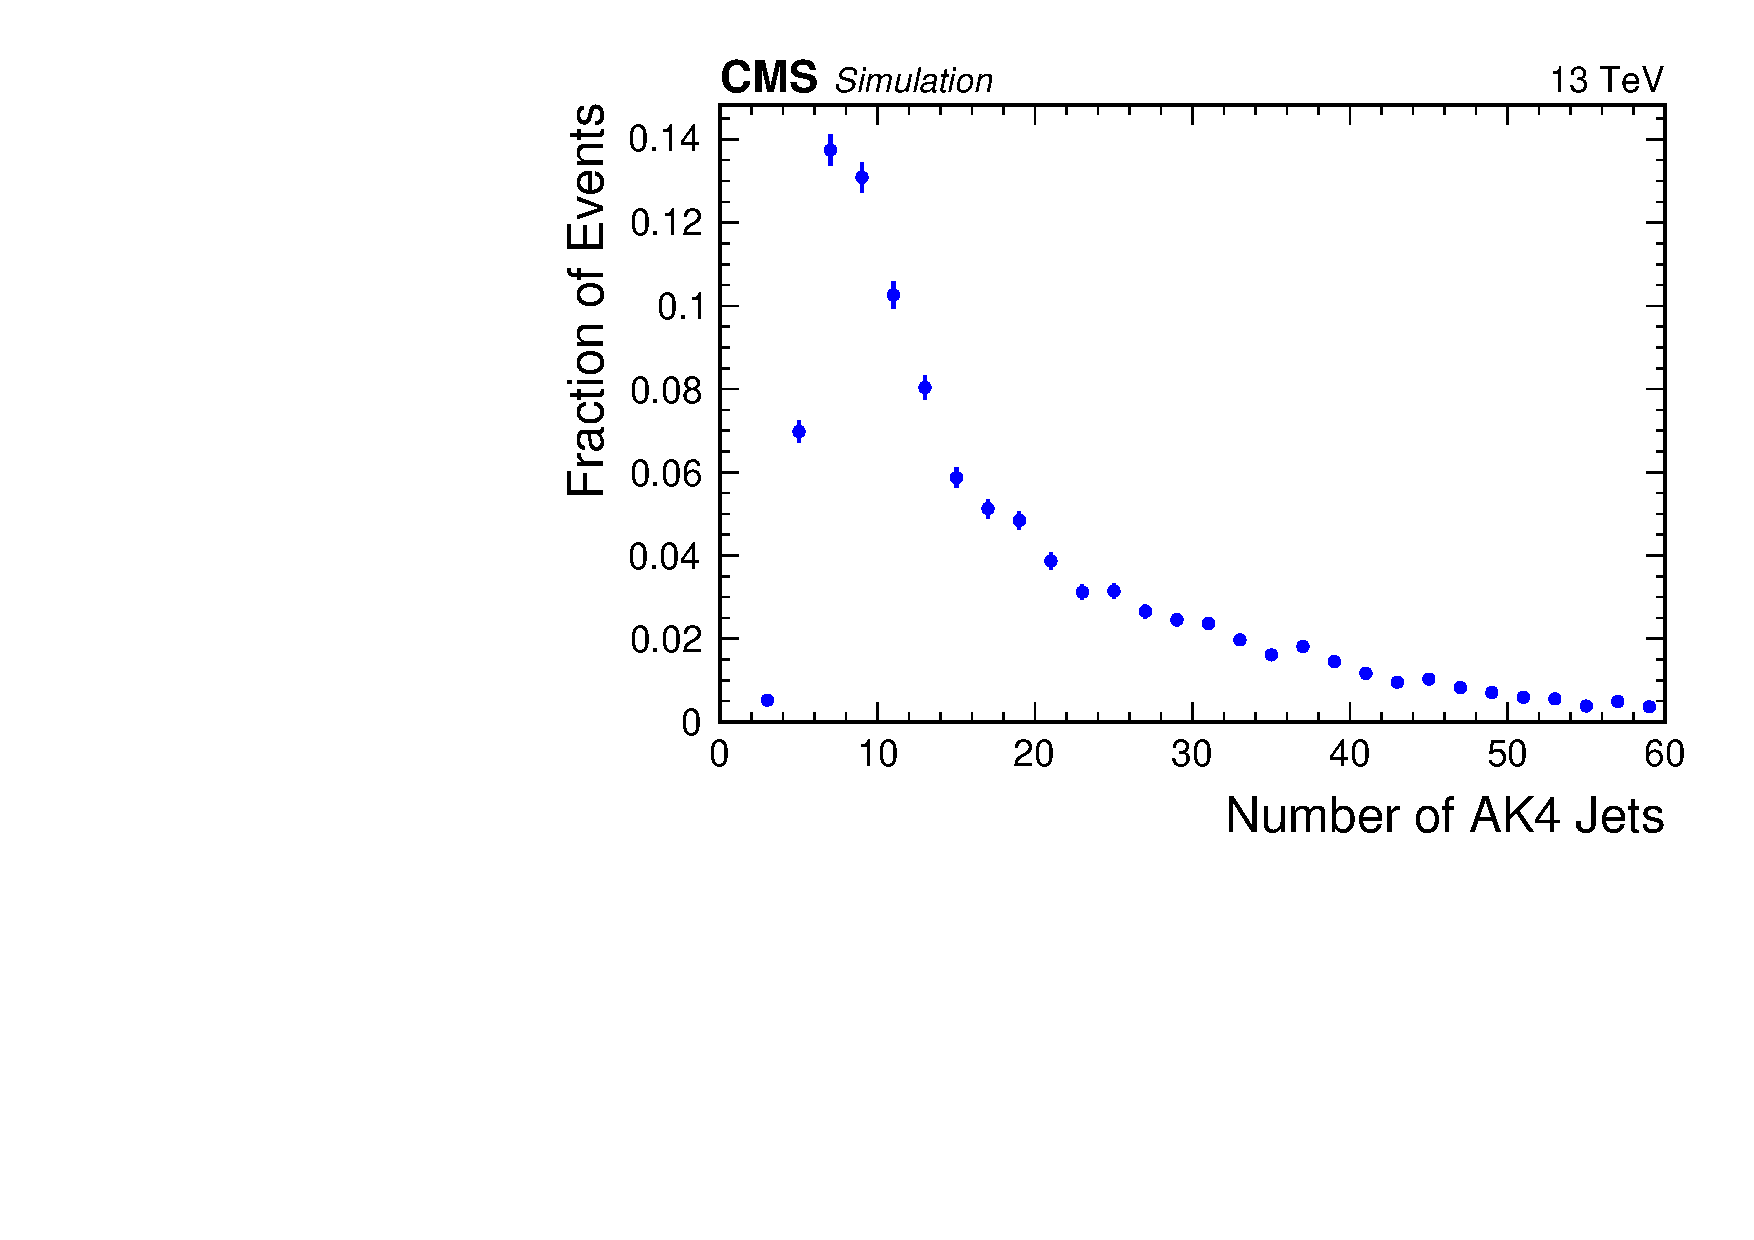
\includegraphics[width=0.32\textwidth]{plots/number_of_ak4jets.pdf}
    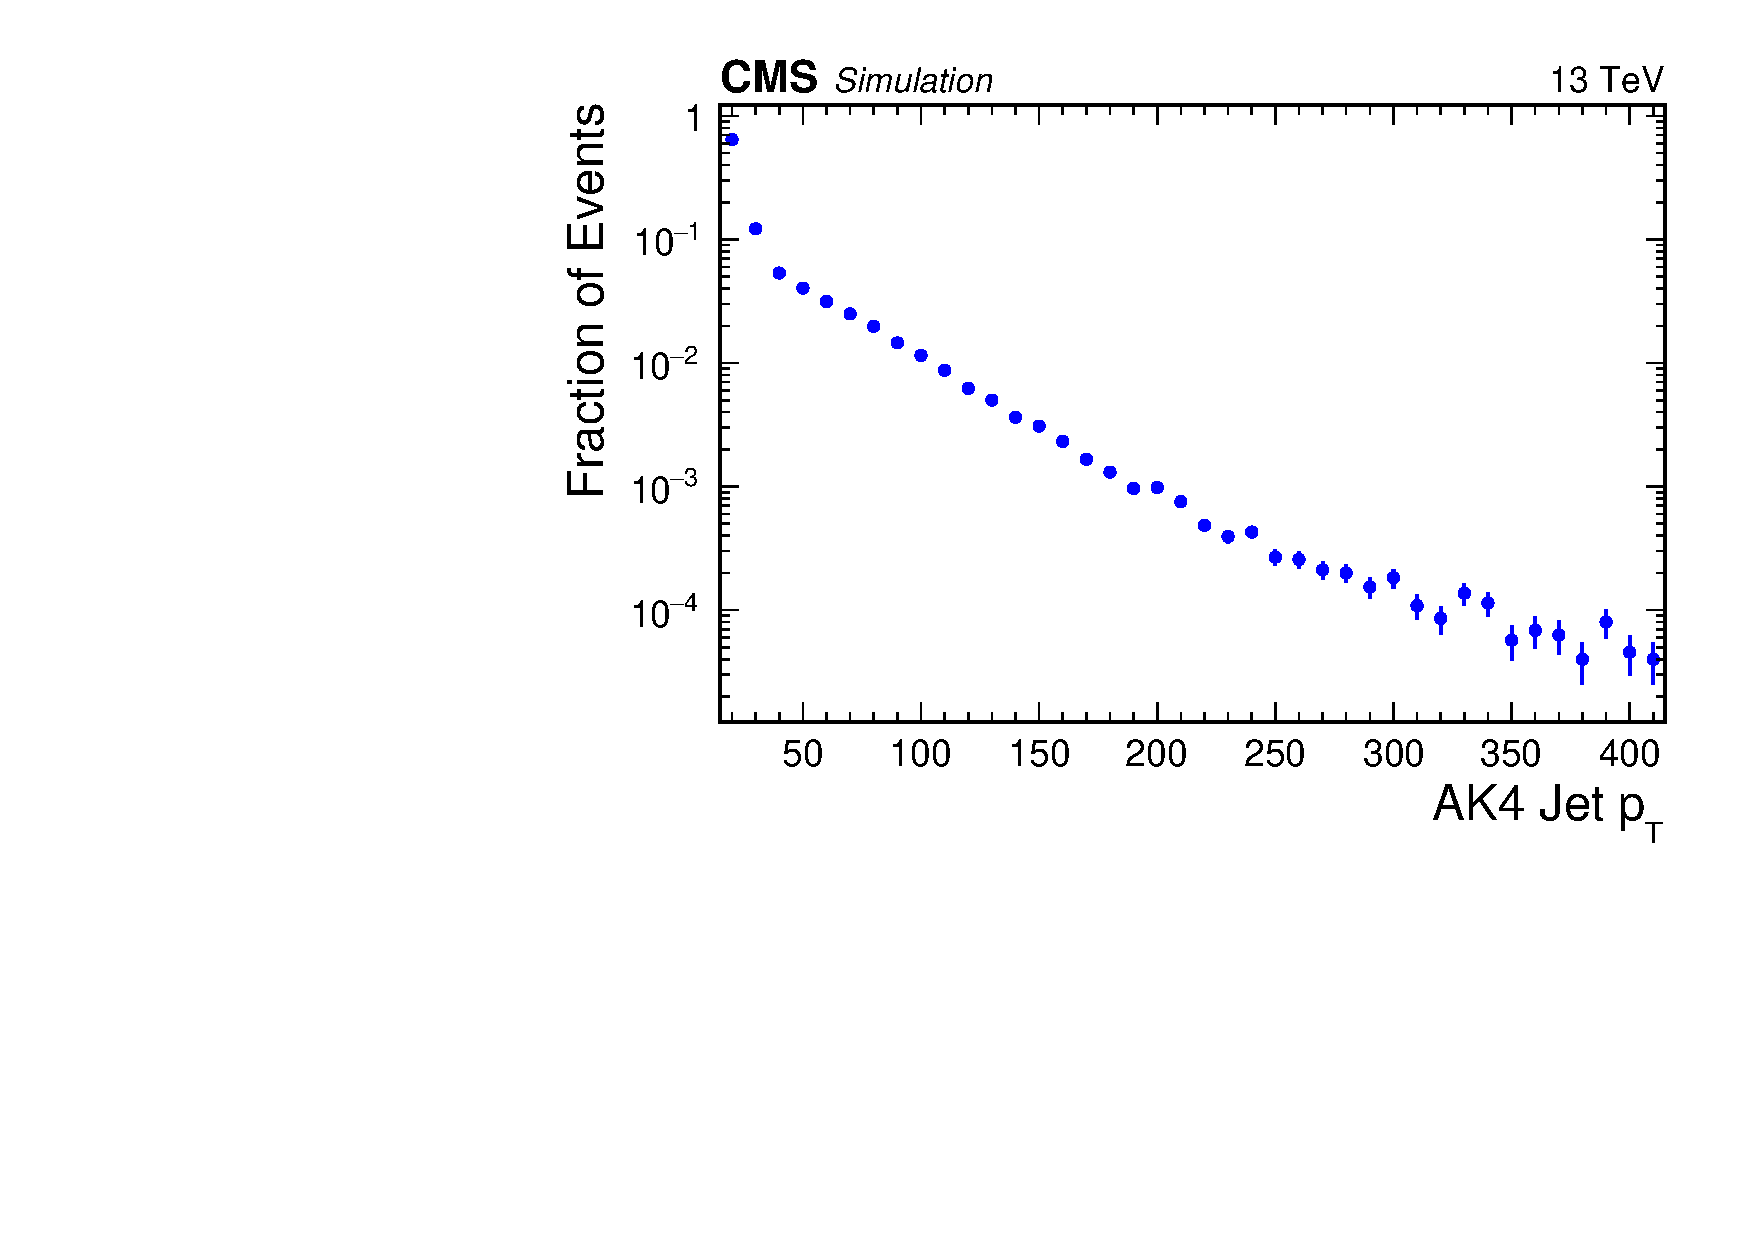
\includegraphics[width=0.32\textwidth]{plots/pt_of_ak4jets.pdf}
    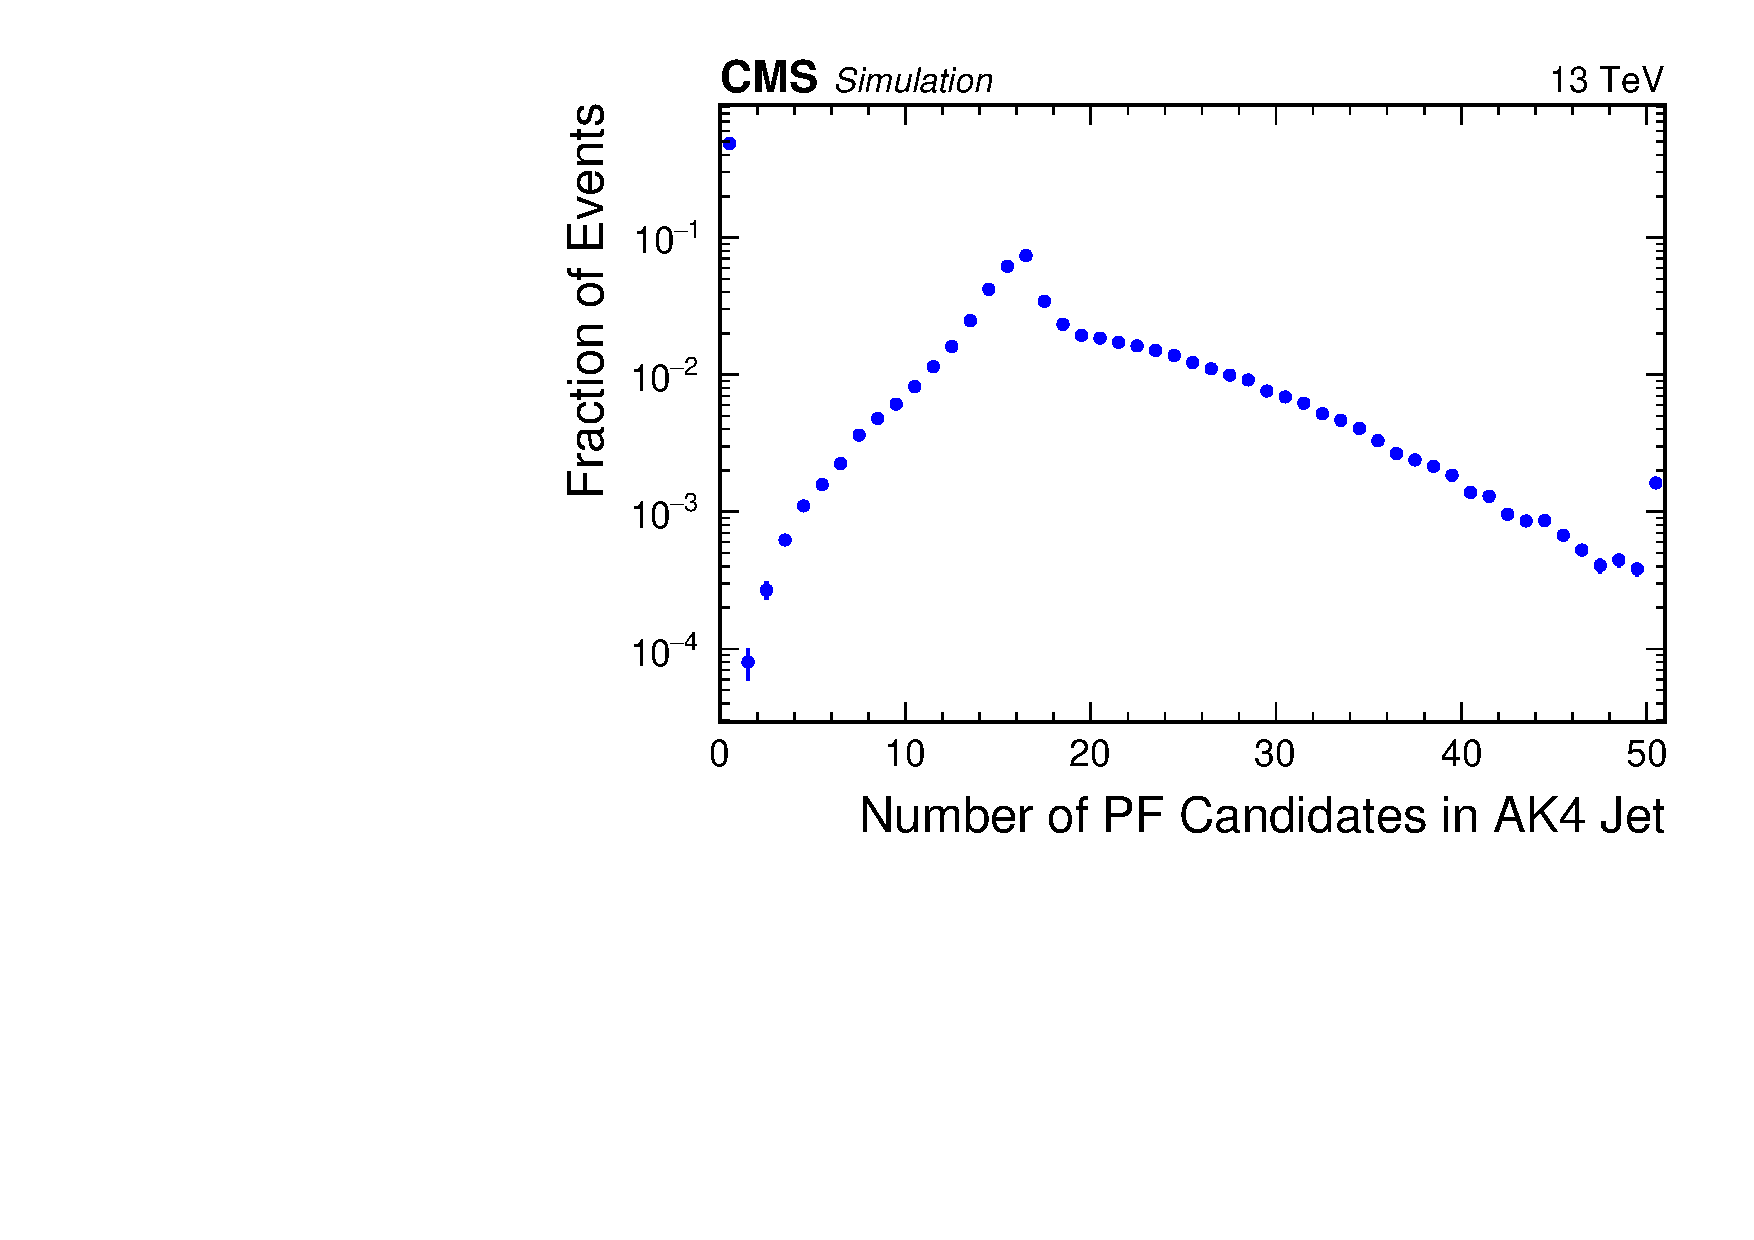
\includegraphics[width=0.32\textwidth]{plots/pfcand_of_ak4jets.pdf}
    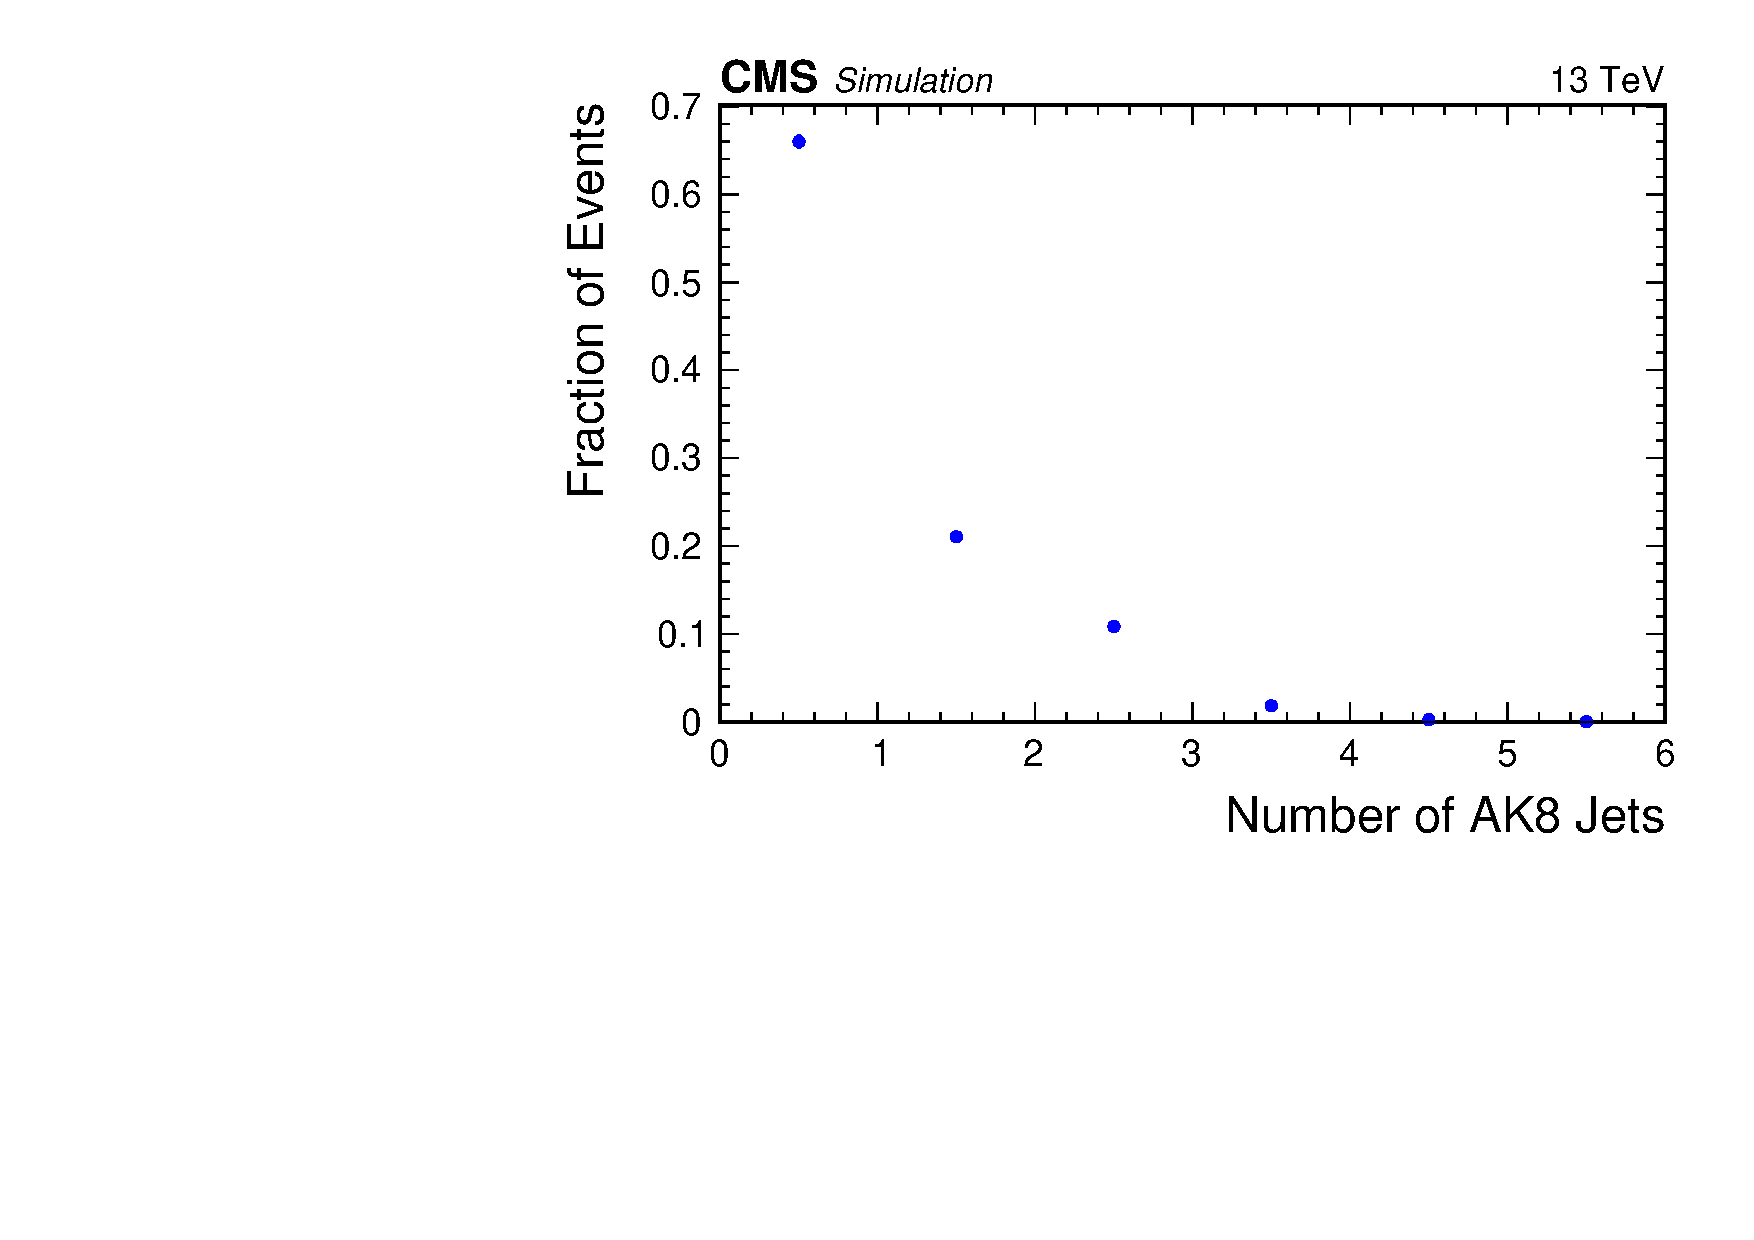
\includegraphics[width=0.32\textwidth]{plots/number_of_ak8jets.pdf}
    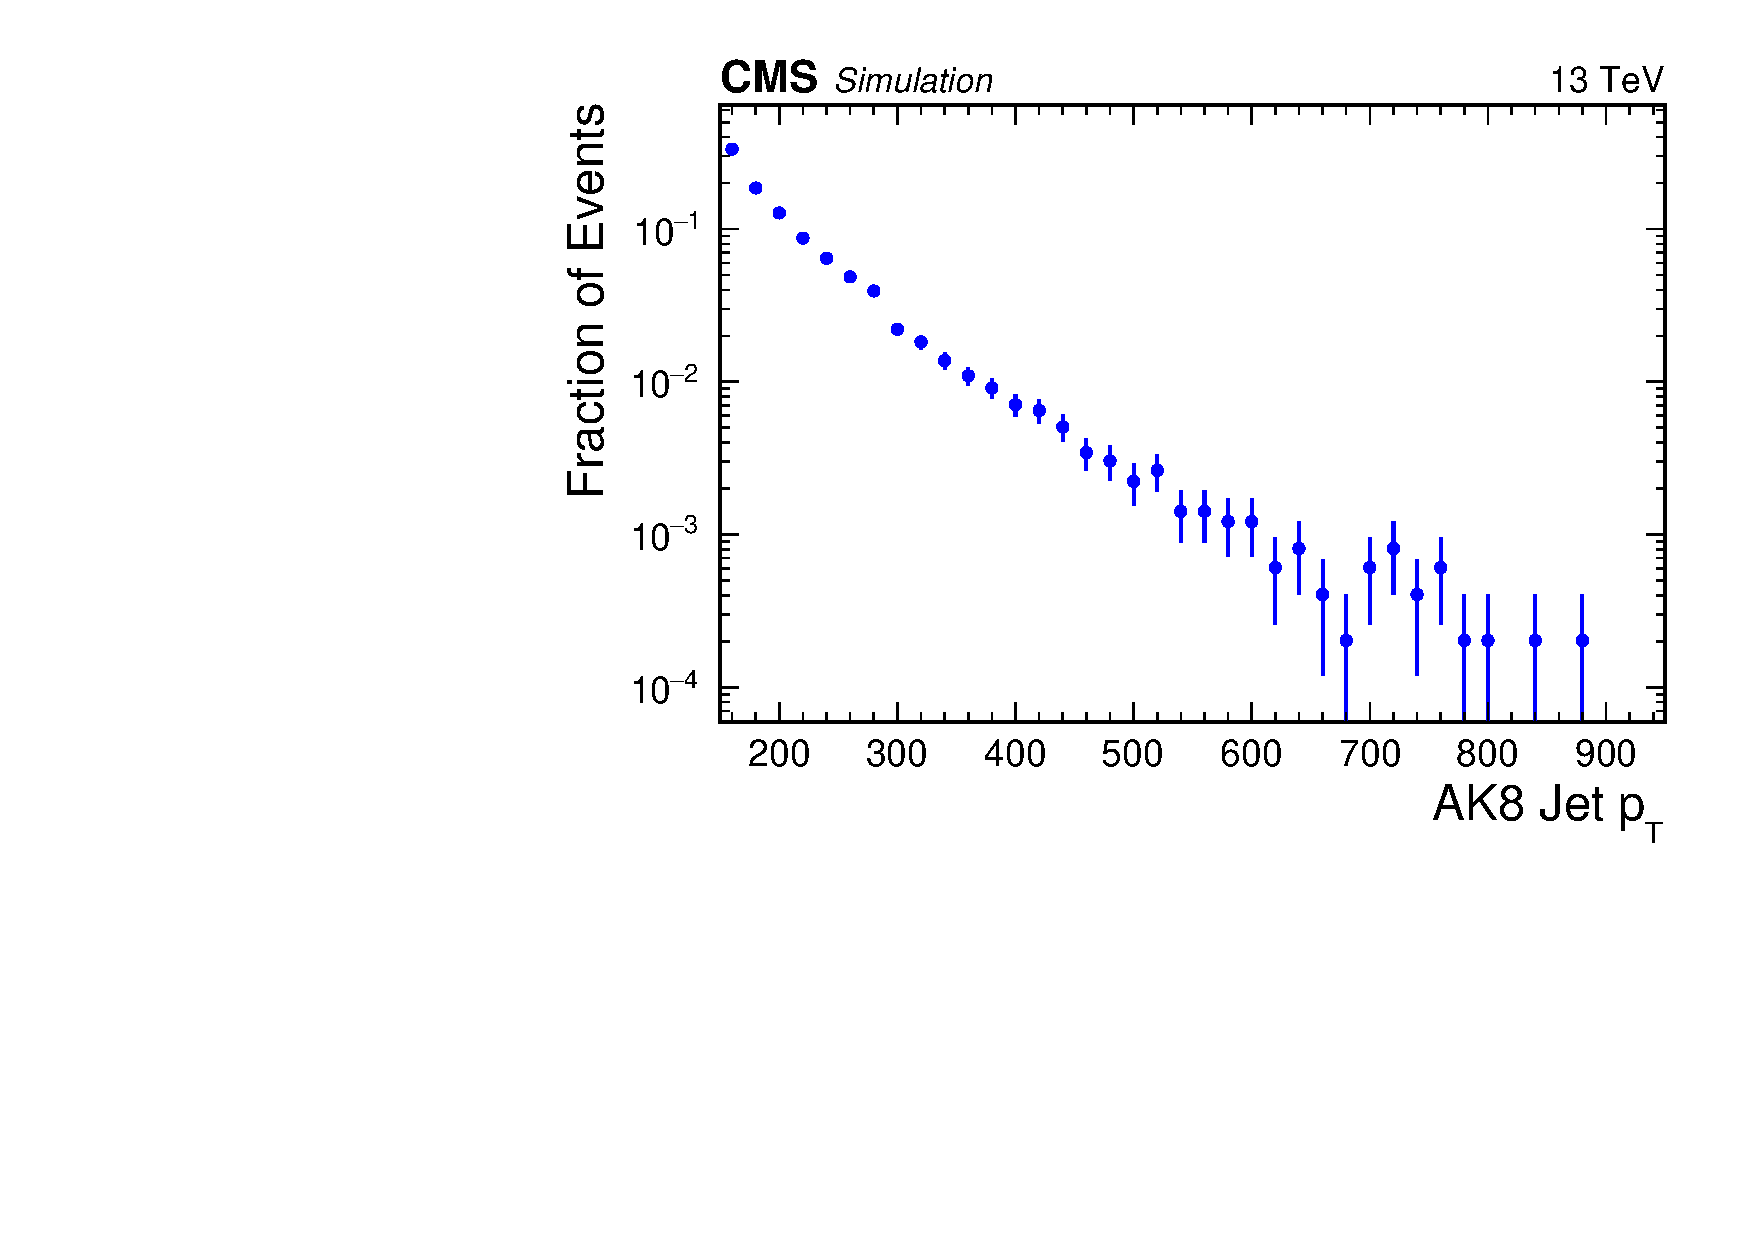
\includegraphics[width=0.32\textwidth]{plots/pt_of_ak8jets.pdf}
    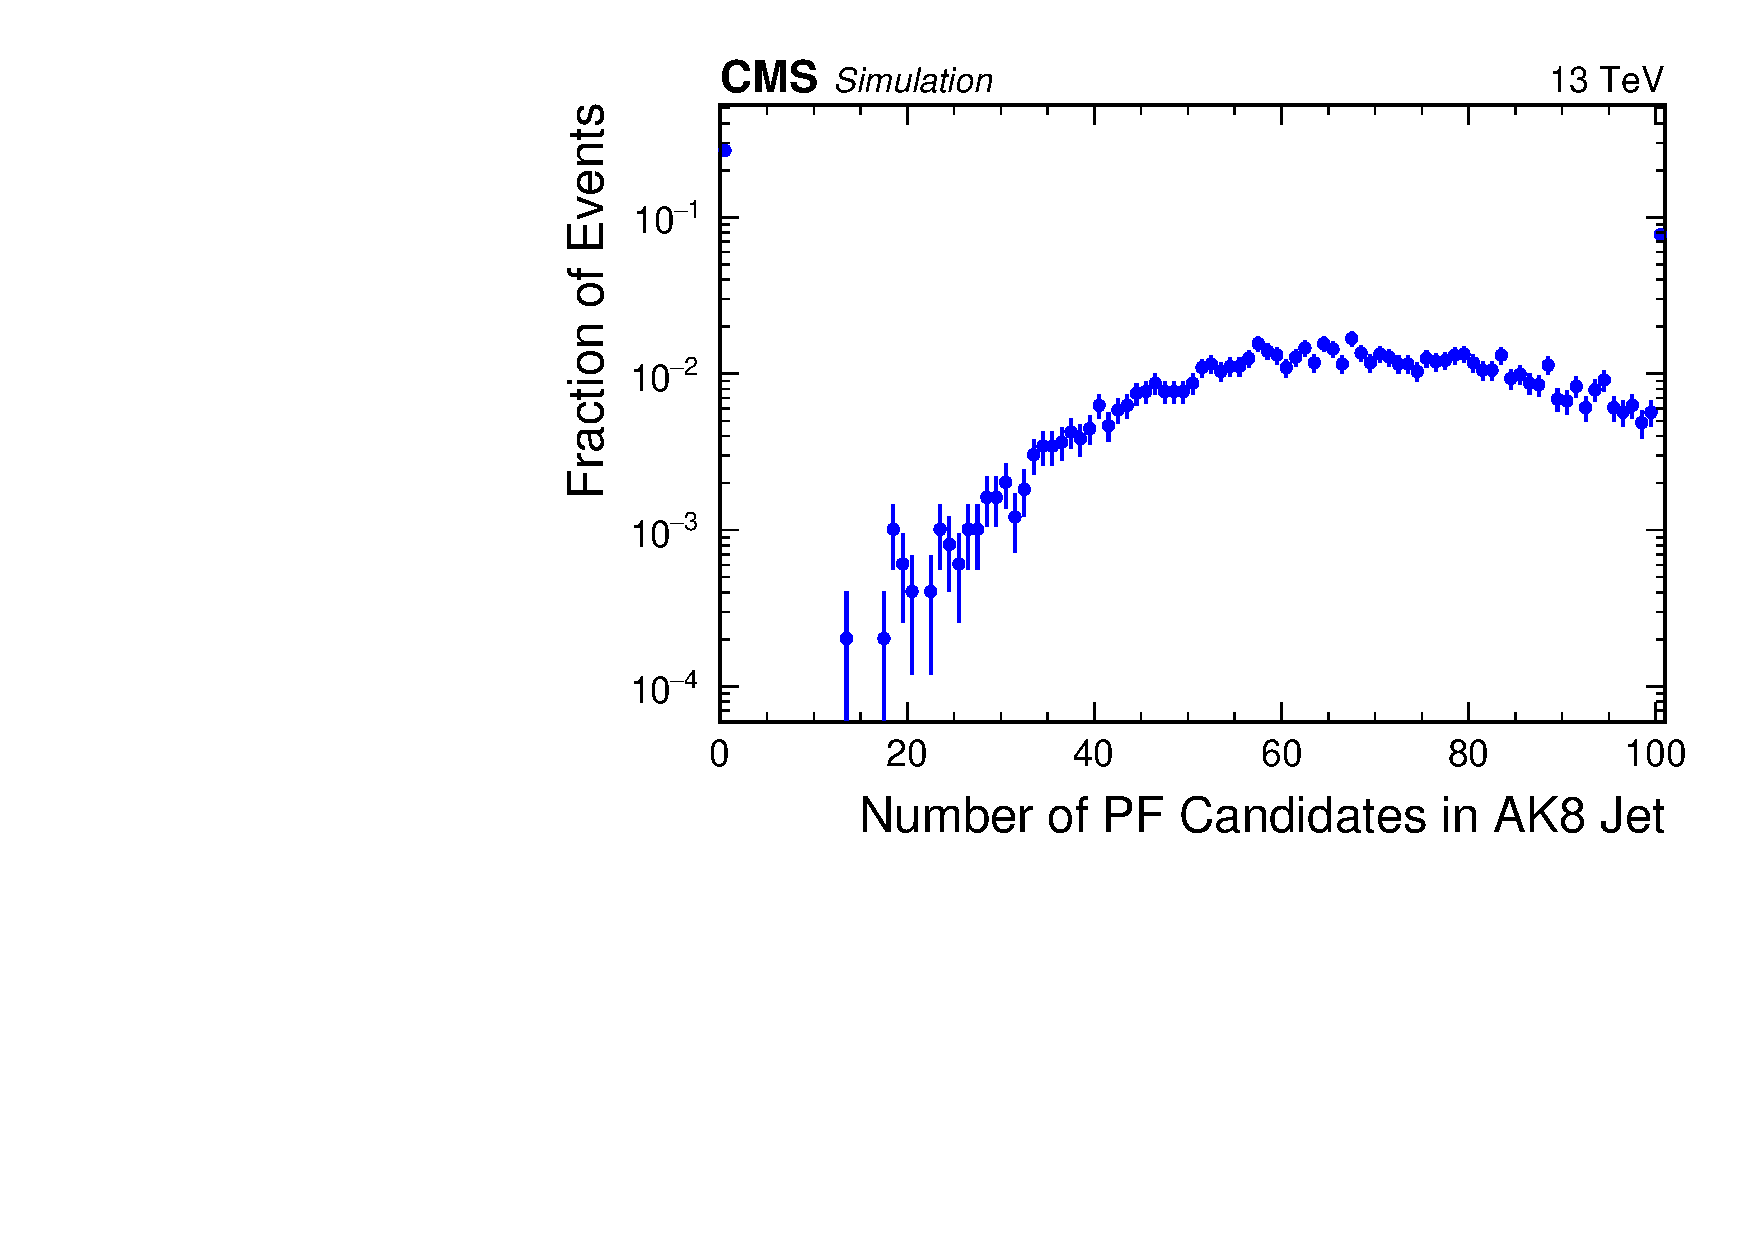
\includegraphics[width=0.32\textwidth]{plots/pfcand_of_ak8jets.pdf}
    \caption{Illustration of the jet information in Run-2 simulated $\ttbar$ dataset used in subsequent studies. The number per event (left), \pt distribution (middle), and distribution of number of particle-flow candidates per jet (right) are shown for AK4 jets (top) and AK8 jets (bottom). In the particle-flow candidate plots, the right-most bin is an overflow bin.}
    \label{fig:jet_content}
\end{figure}

In the configuration where all AK4 jets are padded to 50 particles and 5 vertices and all AK8 jets are padded to 100 particles and 10 vertices, a single 4-threaded job processing a Run 2 \ttbar event will generate about 140\unit{kB/s} of server input for AK4 jets and about 10\unit{kB/s} of server input for each of the AK8 jet versions of PN. At a processing rate of about 4 events per second, with about 16 AK4 jets per event, this corresponds about 2\unit{kB} of information per jet, which is consistent with the number of float inputs per jet.



\subsubsection{DeepMET}
The missing transverse momentum \ptvecmiss is defined as the negative vector sum of the transverse momenta of all the particles in an event, and its magnitude is denoted as \ptmiss~\cite{CMS:2019ctu}. DeepMET (DM)~\cite{DeepMET} is a \TENSORFLOW-based~\cite{tensorflow} deep neural network model that estimates the \ptvecmiss in an event. The vector $\ptvecmiss$ is associated with either the production of neutrinos or potential BSM particles that could propagate through the detector interacting only weakly. The inputs to DM are 11 features from each particle-flow candidate~\cite{CMS:2017yfk} in an event, with zero-padding up to 4\,500 candidates for a given event. This zero-padding is necessary for both the standard version of DM and for its SONIC-enabled implementation; similarly, in both cases, only one inference is made per event. DM outputs two values for each event: the \ptvecmiss components in the $x$ and $y$ directions. Because every event necessarily has the same number of inputs, dynamic batching is automatically available via SONIC, aiding inference efficiency in cases where many client jobs make concurrent requests within a certain time window (as shown in Fig.~\ref{fig:algorithms}, each client thread will make a request about once per second). A single 4-threaded job processing a Run 2 \ttbar event will generate about 1.3\unit{MB/s} of server input for DM.

\subsubsection{DeepTau}
DeepTau (DT)~\cite{CMS:2022prd} is a \TENSORFLOW-based deep neural network model to identify hadronic decayed tau leptons from the jet collections. The inputs to the network include low-level particle features of electrons/photons, muons, and hadrons, and high-level features such as the tau candidate kinematic information. The output is a three-dimensional vector, representing the probability that the candidate originates from a genuine $\tau$, a muon, an
electron, or a quark or gluon jet. In the implementation of direct inference in CMSSW, the network is split into three sub-models. The first two networks process the lower-level input information separately, and the third network combines the information from the first two models with the high-level information and outputs the discriminator values. In the SONIC implementation, we use a combined model with zero-padded inputs, so that dynamic batching can be used and GPUs can be utilized more efficiently. A single 4-threaded job processing a Run 2 \ttbar event will generate about 4.7\unit{MB/s} of server input for DT, making it the most demanding algorithm explored in this study in terms of server input.
    
    %\item ECAL DRN maybe?  Maybe put that as a separate bullet or just put that in a separate section entirely

\subsection{Latency}
The latency is defined as the real time spent between starting and finishing processing one event. The latency breakdown for the three algorithms highlighted above in the Run-2 \ttbar events is presented in Table~\ref{table:SONIC_Algos}. The per-event average processing time is about 1 second; PN consumes about 6\% of this time, while DM and DT take about 1\% and 2\%, respectively. Thus, for this sample of events, the SONIC-ported algorithms account for about 10\% of the total latency. It is worth noting that this fraction is sample-dependent; for example, if a sample has fewer jets per event, PN will consume a smaller fraction of the per-event latency. However, thanks to the excellent performance of ML algorithms, more and more algorithms used in CMS data processing are being converted to ML versions. These will all benefit from the use of coprocessors, meaning that a higher fraction of latency will be able to be accelerated with SONIC easily in the future.

\begin{table}[ht!]
\begin{center}
\begin{tabular}{c r r r}
 Algorithm & \multicolumn{1}{c}{Time [ms]} & \multicolumn{1}{c}{Fraction [\%]} & \multicolumn{1}{c}{Input [MB]}\\ %[0.5ex] 
 \hline
 ParticleNet & 62.1 & 6.3 & 0.05 \\
 DeepMET & 13.2 & 1.3 & 0.33 \\
 DeepTau & 21.1 & 2.1 & 1.18 \\
 \hline
 PN+DM+DT & 96.4 & 9.7 & 1.56 \\ 
 \hline
 Total & 993.3 & 100.0 & -- \\ 
\end{tabular}
\caption{The latency of the Mini-AOD processing illustrated in Fig.~\ref{fig:algorithms}, which does not use SONIC. The latency of the algorithms for which a SONIC version was created are stated explicitly. They consume about 10\% of the total per-event latency. This table also contains the expected server input for each model type created per event in Run 2 \ttbar events.}
\label{table:SONIC_Algos}
\end{center}
\end{table}

\subsection{Computing resources}

Fermilab, via the LHC Physics Center (LPC), provides CPU-only batch resources and a set of interactive machines with NVIDIA Tesla T4 GPUs. Through Fermilab, we were also able to steer the allocation of cloud resources (see below) using the HepCloud~\cite{Holzman:2017jgg} framework. These resources are physically located in Illinois.
%need to be more specific?

The Google Cloud Platform (GCP) provides CPU-only virtual machines (VMs) and VMs enabled with NVIDIA Tesla T4 GPUs. By default, the CPUs are a mix of Skylake, Broadwell, Haswell, Sandy Bridge, and Ivy Bridge architectures. In GCP, we created customized machines with specified numbers of CPU threads or different ratios of CPU threads to number of GPUs. Similarly, a customized, dynamic SLURM~\cite{slurm} cluster was created that could instantiate and deplete 4-thread VMs on demand for medium-scale tests that ran jobs across $\mathcal{O}(1000)$ CPUs. The cluster's 4-thread configuration was chosen so that 4-threaded CMSSW jobs would saturate the node's resources, improving reproducibility of timing tests. CPU-only VMs could also be instantiated through HepCloud. In GCP, we also maintained GPU-enabled VMs running Triton servers that both the SLURM and HepCloud client nodes could access. These resources are physically located in Iowa.

At the Purdue CMS Tier-2 computing cluster, tests were performed with reserved CPU-only and GPU-enabled machines. The CPU-only machines are 20-core Intel E5-2660 v3 machines, and the GPU-enabled machines each have two AMD EPYC-7702 CPUs with a NVIDIA Tesla T4 GPU. Reserving these nodes allowed for controlled resource utilization, leading to more reproducible timing tests. These resources are physically located in Indiana.

It is important to note that having a diversity of locations for these resources allows for a clear demonstration of one of SONIC's key features, namely that it enables the use of non-local resources. We were able to start a server in one location and have client jobs running at another site. One such study will be presented in Section~\ref{sec:different_sites}.


%\subsection{Ragged batching}
%\label{sec:ragged}

%In the SONIC paradigm, it is generally easiest to make one inference request per event for each model hosted as-a-service. For some models, such as PN, this entails making inference requests with batch size greater than 1, involving multiple objects with potentially different numbers of inputs. This introduces a subtlety with respect to padding. Older versions of Triton did not allow for ``ragged batching'', in which inference requests for models with a variable number of inputs can be combined into a single batch even if each request has a different number of inputs. Because of this, two approaches can be taken.

%In a maximally-padded approach, every object would be padded to the same input size. For example, in PN each jet can be padded to 100 particles and 10 vertices. In this scenario, all inference requests, including those for different events, will have the same number of inputs, making dynamic batching across events possible. This maximally-padded case will consume unnecessary bandwidth, as a significant fraction of the data transfer will be padding.

%To get around this, one can implement a ``pseudo-ragged'' version of models, where objects in an event are padded up to the largest size of a single object in that event. For the PN example, this means that jets in an event would be padded up to the number of particles and vertices found in the largest jet in its event. This reduces wasted bandwidth for a given request---for the Run 2 \ttbar sample explored here, the input bandwidth is reduced by about a factor of 2 overall. In this case, Triton will batch together jets from the same event, and if by some coincidence, two separate inference requests were made for events with the same maximal jet size, then dynamic batching between the inferences would be possible. However, that is rare, so in practice pseudo-ragged PN does not take advantage of dynamic batching.

%In the large-scale Mini-AOD production tests described below, the benefits of dynamic batching make the maximally-padded scenario favorable in terms of latency reduction, as many client jobs will be making requests concurrently, and batching is beneficial to inference efficiency. In scenarios where only one or a few client jobs are running at once for a given server, then the pseudo-ragged version provides superior throughput. Recent releases of Triton started supporting ragged batching, which is a feature under study and benchmarks.


\section{Performance}
\label{sec:performances}
In this section we discuss the performance of running Mini-AOD productions with SONIC. The comparisons are done with respect to ``direct" inference, which refers to the current standard approach where the ML inference backends are integrated into \CMSSW and everything runs inside \CMSSW on CPUs. 

As mentioned in Sec.~\ref{sec:triton}, since there are some degrees of freedom when deploying the models on the server, first we start with the per-algorithm optimizations in order to find the optimal algorithm configuration for productions. Then we check the impacts of deploying servers on different sites. Finally we mimic the real productions by running the scale-up tests and check the performances.

\subsection{Per-algorithm Inference Optimization}
\label{sec:algo_acceleration}
%We measure the throughputs and latency of the ParticleNet algorithm on one NVIDIA Tesla T4 GPU, with different inference backends supported in Triton: ONNX, Pytorch, and also Pytorch with TensorRT optimizations. The results are shown in Fig.~\ref{fig:throughputs_pn}.

To maximize the resource efficiency and throughput benefits of SONIC, it is necessary to start with some single-model characterization studies out of \CMSSW. For example, in order to maximize GPU usage without oversaturation, we need to find the optimal ratio of client-side CPUs to server-side GPUs, find the best batch size for inference in the Triton server, and choose the model configuration that will give the best throughput.

The latter two optimizations can be performed with the Triton Model Analyzer tool~\cite{triton_model_analyzer}. This tool feeds certain inputs in the correct tensor format to a loaded model hosted on a server, allowing for robust characterization of latency per inference or exploration of the impact of batch size.
As an example, we measure the latency and throughput of the ParticleNet (PN) algorithm for AK4 jet tagging on one NVIDIA Tesla T4 GPU, with different inference backends supported in Triton: \ONNX, \ONNX with TRT, and \PYTORCH~\cite{pytorch}. %Was this done at Purdue?
The results are shown in Fig.~\ref{fig:throughputs_pn}. 

\begin{figure}[ht]
    \centering
    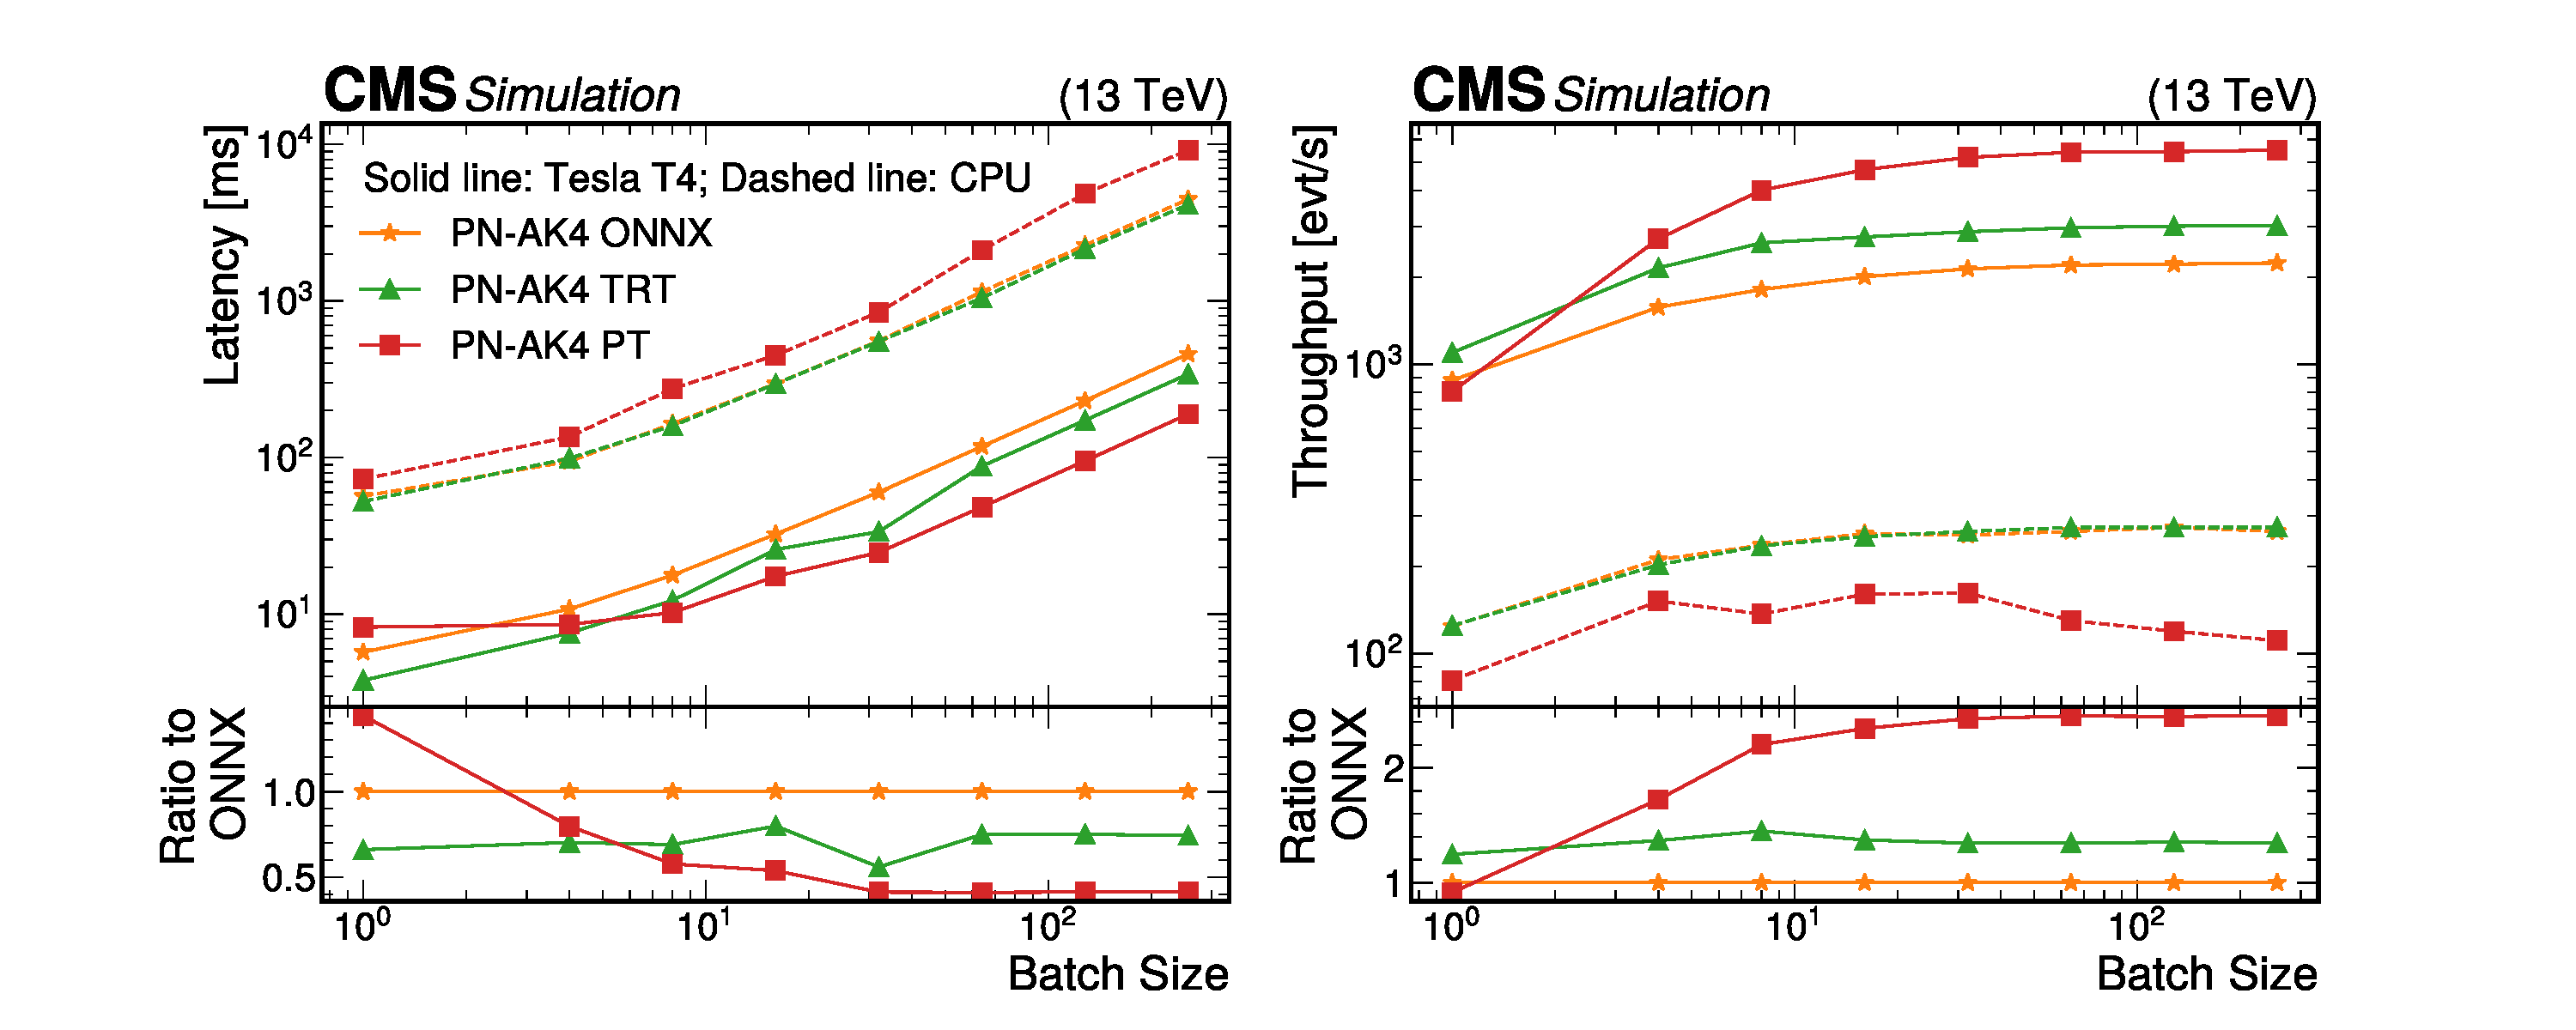
\includegraphics[width=0.98\textwidth]{plots/latencies_throughputs_pn.pdf}
    \caption{Latency (left) and throughput (right) of the AK4 ParticleNet algorithm serviced by a Triton server running on one NVIDIA Tesla T4 GPU, presented as a function of the batch size. Values are shown for different inference backends: \ONNX (orange), \ONNX with TRT (green), and \PYTORCH (red). Performance for these backends when run on a CPU-based Triton server are given in dashed lines, with the same color-to-backend correspondence.}%(\textcolor{red}{Plot will be updated; need to include some benchmarks of the throughputs and latency measured on CPUs as a function of batch size.})}
    \label{fig:throughputs_pn}
\end{figure}

For smaller batch sizes, the TRT version of PN algorithm leads to the highest throughput in total inferences per second, while at higher batch sizes, the \PYTORCH version gives higher throughput. In the SONIC-enabled version of PN in CMSSW, all of the jets in a single event are batched together, and there are typically about 16 AK4 jets per event in our \ttbar sample. To achieve higher batch sizes in a production scenario, multiple jobs would need to make an inference request from the same server within a relatively narrow time window. Triton allows us to specify a preferred batch size, such that if many inference request are queued in quick succession, the server will try to perform inferences with batches of approximately the specified size. For example, the peak throughput seems to plateau around a batch size of 100 for the \PYTORCH version of PN.%be achieved at a batch size of 60 for the PyTorch version of PN.
%WHICH VERSION OF PN DID WE END UP USING?  TRT?
%IN THE FIGURE, IS THAT REALLY EVENTS PER SECOND?  OR IS THAT INFERENCES PER SECOND
%What is our batching window?

Similar studies can be performed on other models as well. Fig.~\ref{fig:throughputs_deepmet} and~\ref{fig:throughputs_deeptau} show the latency and throughput scans of DeepMET and DeepTau models. 

\begin{figure}[ht]
    \centering
    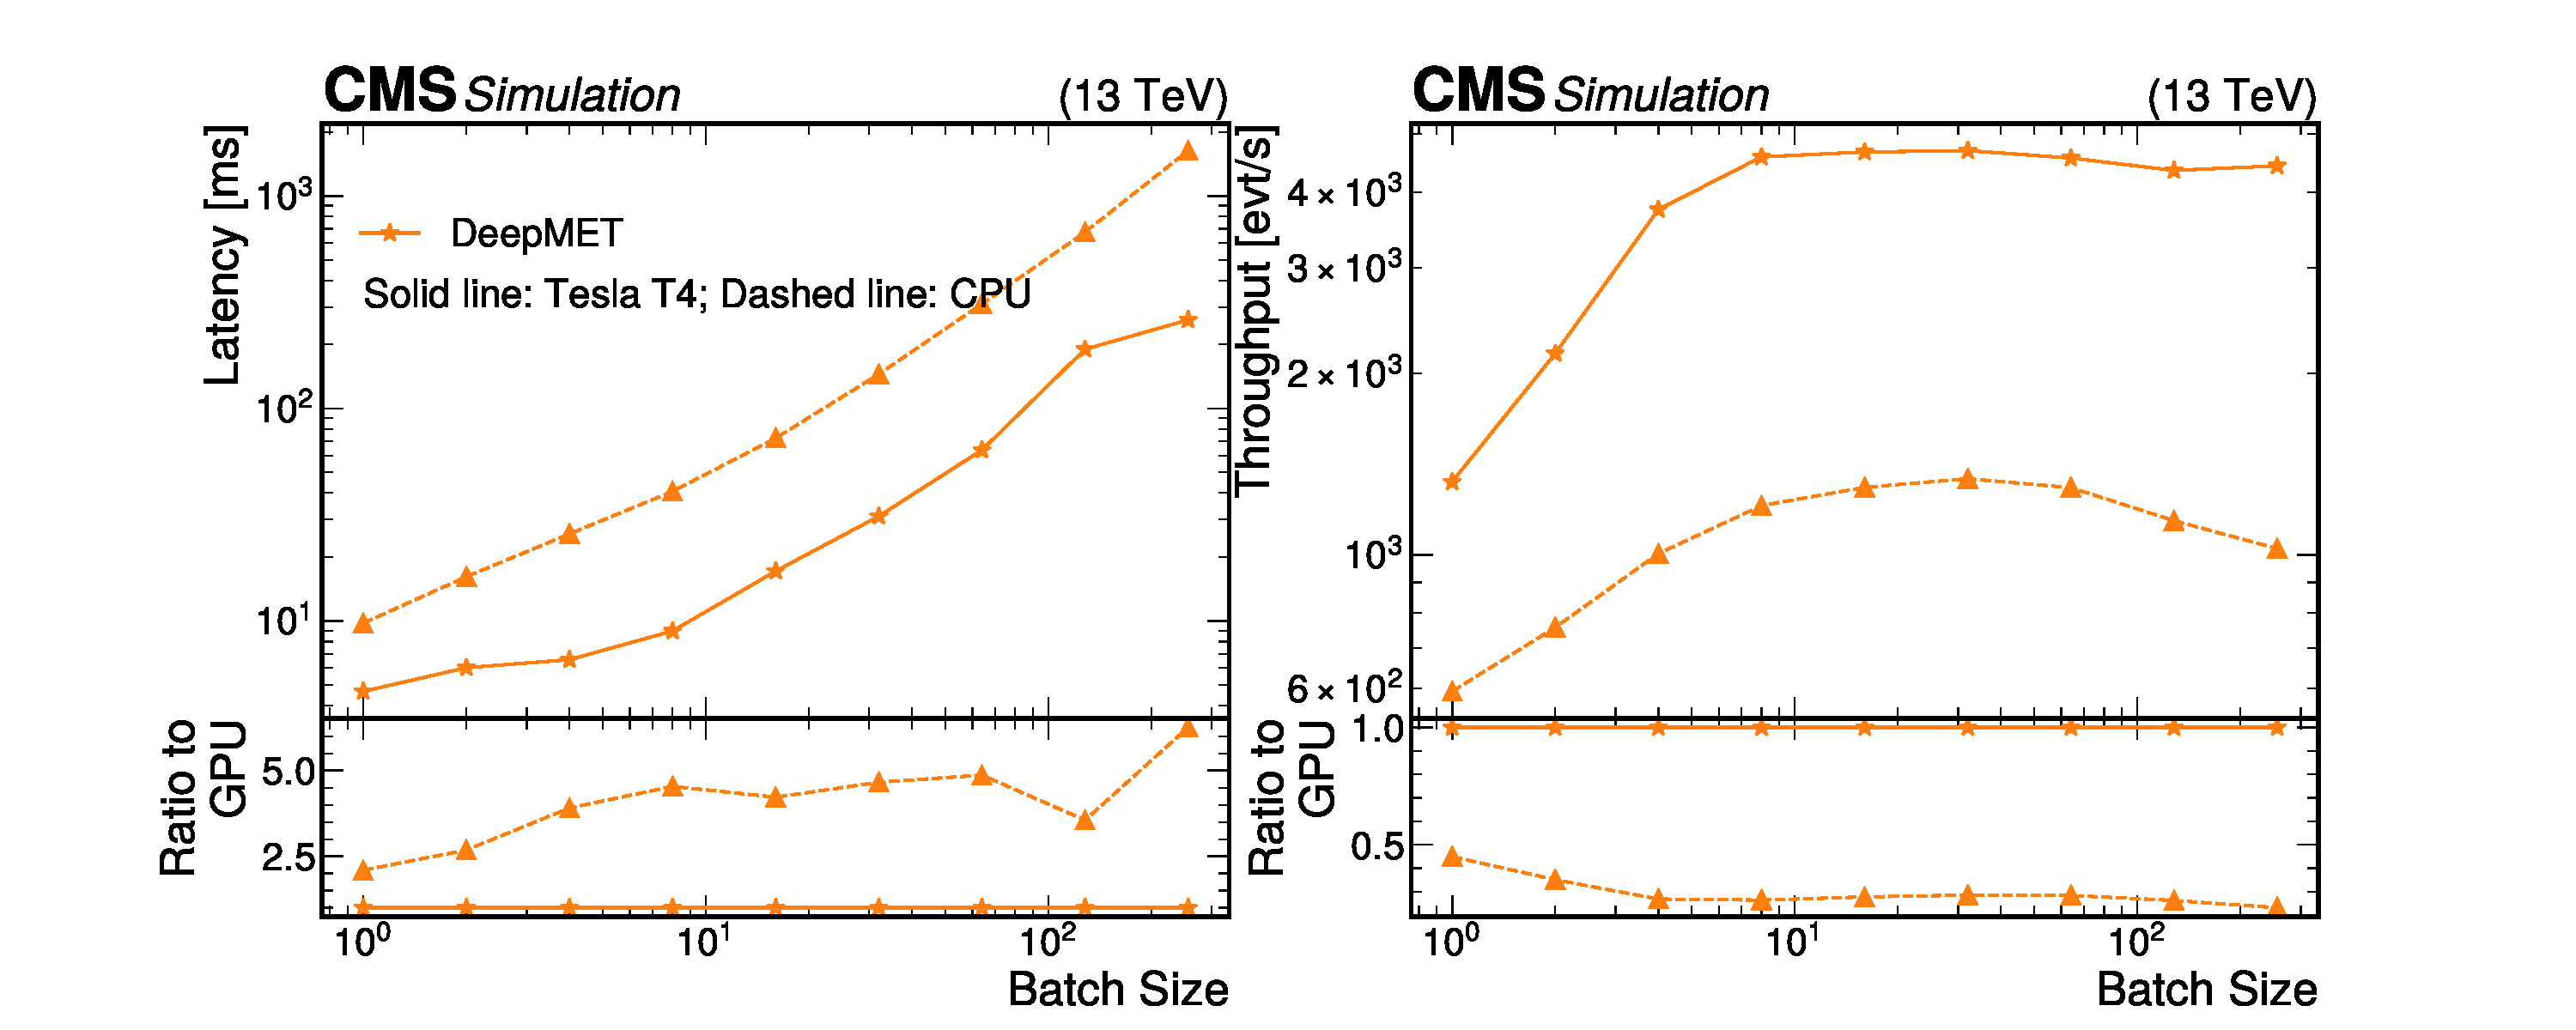
\includegraphics[width=0.98\textwidth]{plots/latencies_throughputs_deepmet.pdf}
    \caption{Latency (left) and throughput (right) of the DeepMET algorithm serviced by a Triton server running on one NVIDIA Tesla T4 GPU, presented as a function of the batch size. Values are shown for different inference backends: \TENSORFLOW (orange), and \TENSORFLOW with TRT (green). Performance for these backends when run on a CPU-based Triton server are given in dashed lines, with the same color-to-backend correspondence.}%
    \label{fig:throughputs_deepmet}
\end{figure}

\begin{figure}[ht]
    \centering
    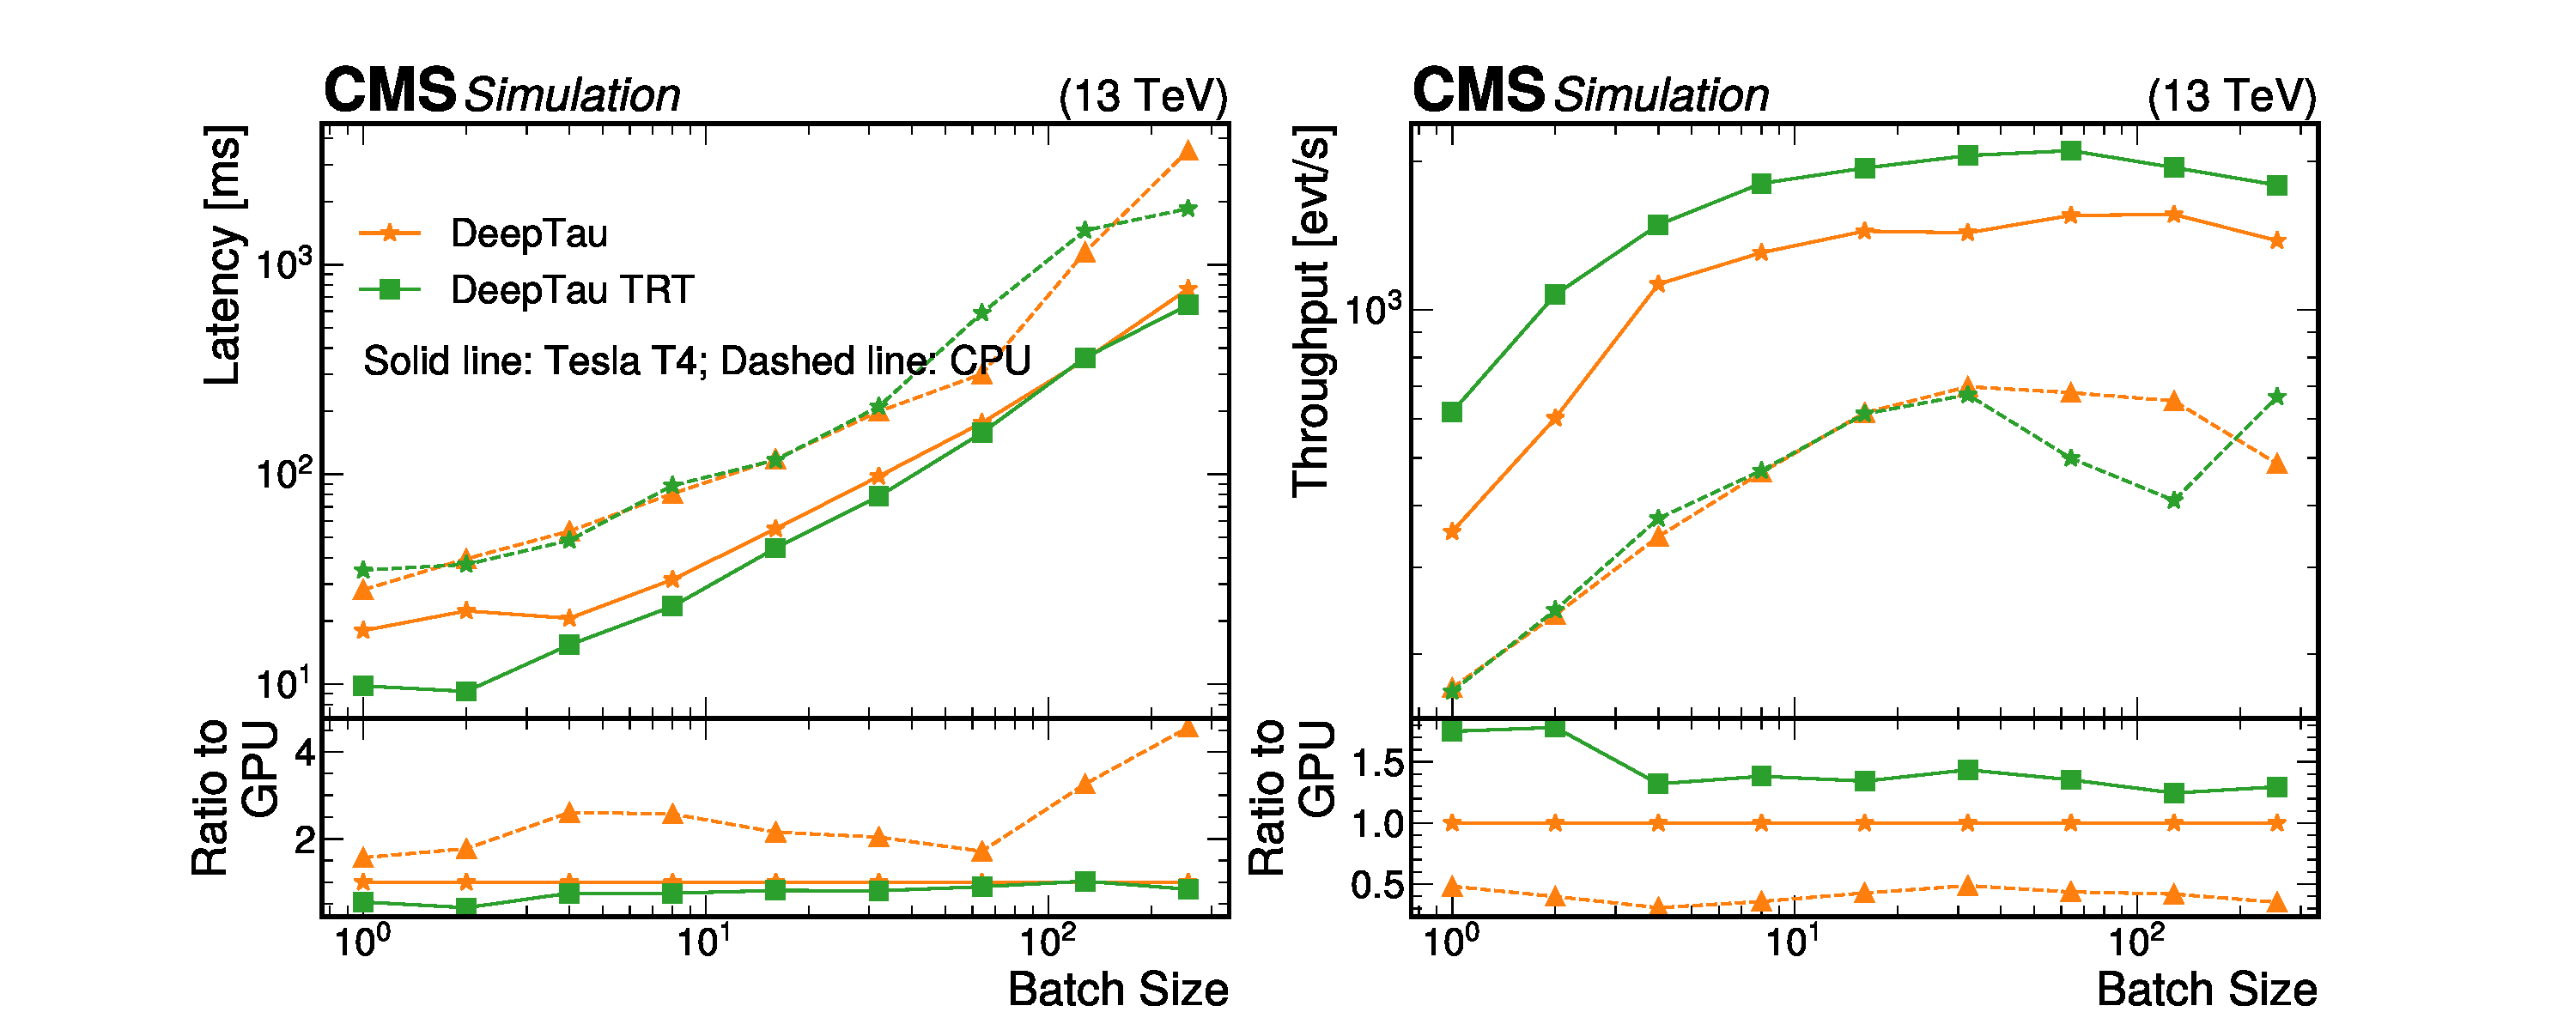
\includegraphics[width=0.98\textwidth]{plots/latencies_throughputs_deeptau.pdf}
    \caption{Latency (left) and throughput (right) of the DeepTau algorithm serviced by a Triton server running on one NVIDIA Tesla T4 GPU, presented as a function of the batch size. Values are shown for different inference backends: \TENSORFLOW (orange), and \TENSORFLOW with TRT (green). Performance for these backends when run on a CPU-based Triton server are given in dashed lines, with the same color-to-backend correspondence.}%
    \label{fig:throughputs_deeptau}
\end{figure}

The model analyzer can also approximately determine how many inferences per second a single GPU can perform before saturation. For example, for the \PYTORCH version of PN for AK4 jets, a single Tesla T4 GPU can perform about 6\,000 inferences per second without saturating. This corresponds to about 400 \textit{events} per second, given the typical number of jets per event.
Based on this, we can estimate how many CPU clients one GPU can support in parallel. A typical production configuration runs 4-threaded Mini-AOD jobs, each of which processes about 3.6 events per second. Therefore, a single GPU should be able to handle about 110 4-threaded jobs in parallel running asynchronously, assuming it is being used exclusively for a single server hosting the PyTorch AK4 PN model.

This expected saturation point can be tested directly by scanning the throughput as a function of the number of CPU clients pinging one GPU server. Figure~\ref{fig:throughputs_scan_pn} shows such tests for AK4 PN, the AK8 PN models, DeepMET, and DeepTau, which were performed in GCP using a custom SLURM cluster. For each model, a single server running on one NVIDIA T4 GPU was started on one cloud VM, and client-side jobs were executed in VMs that had 4 CPU threads. The tests for each model class were performed separately, and as one model class was being tested, the non-SONIC versions of the other models were used.
When offloading PN inference to GPU, we expect an improvement in the overall throughput of about 5\% compared with direct inferences, corresponding to the fraction of time taken by the total AK4 PN processing. Such an improvement is observed before saturation, where the throughput is stable as a function of the number of simultaneous CPU clients. The throughput decreases as the GPU starts to saturate, as individual client-side jobs have to wait longer for inference requests to complete and return. The throughput becomes slower than CPU-only inference at a bit after 160 parallel jobs. This is a bit higher than the prediction from the model analyzer, likely due to the fact that the majority of the real input is padded 0s, while the model analyzer uses randomized input.
\begin{figure}[ht]
    \centering
    %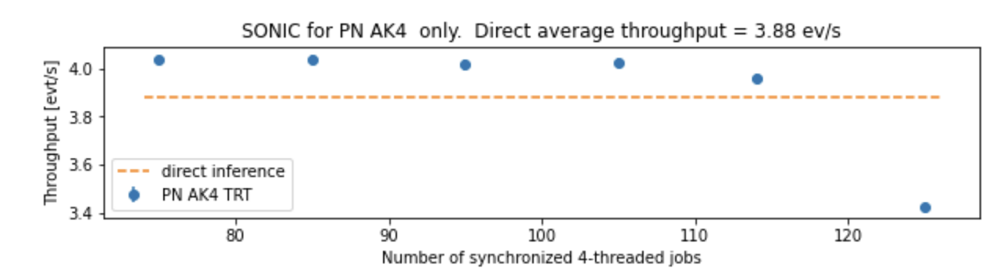
\includegraphics[width=0.90\textwidth]{plots/throughput_njobs_scan_pn.png}
    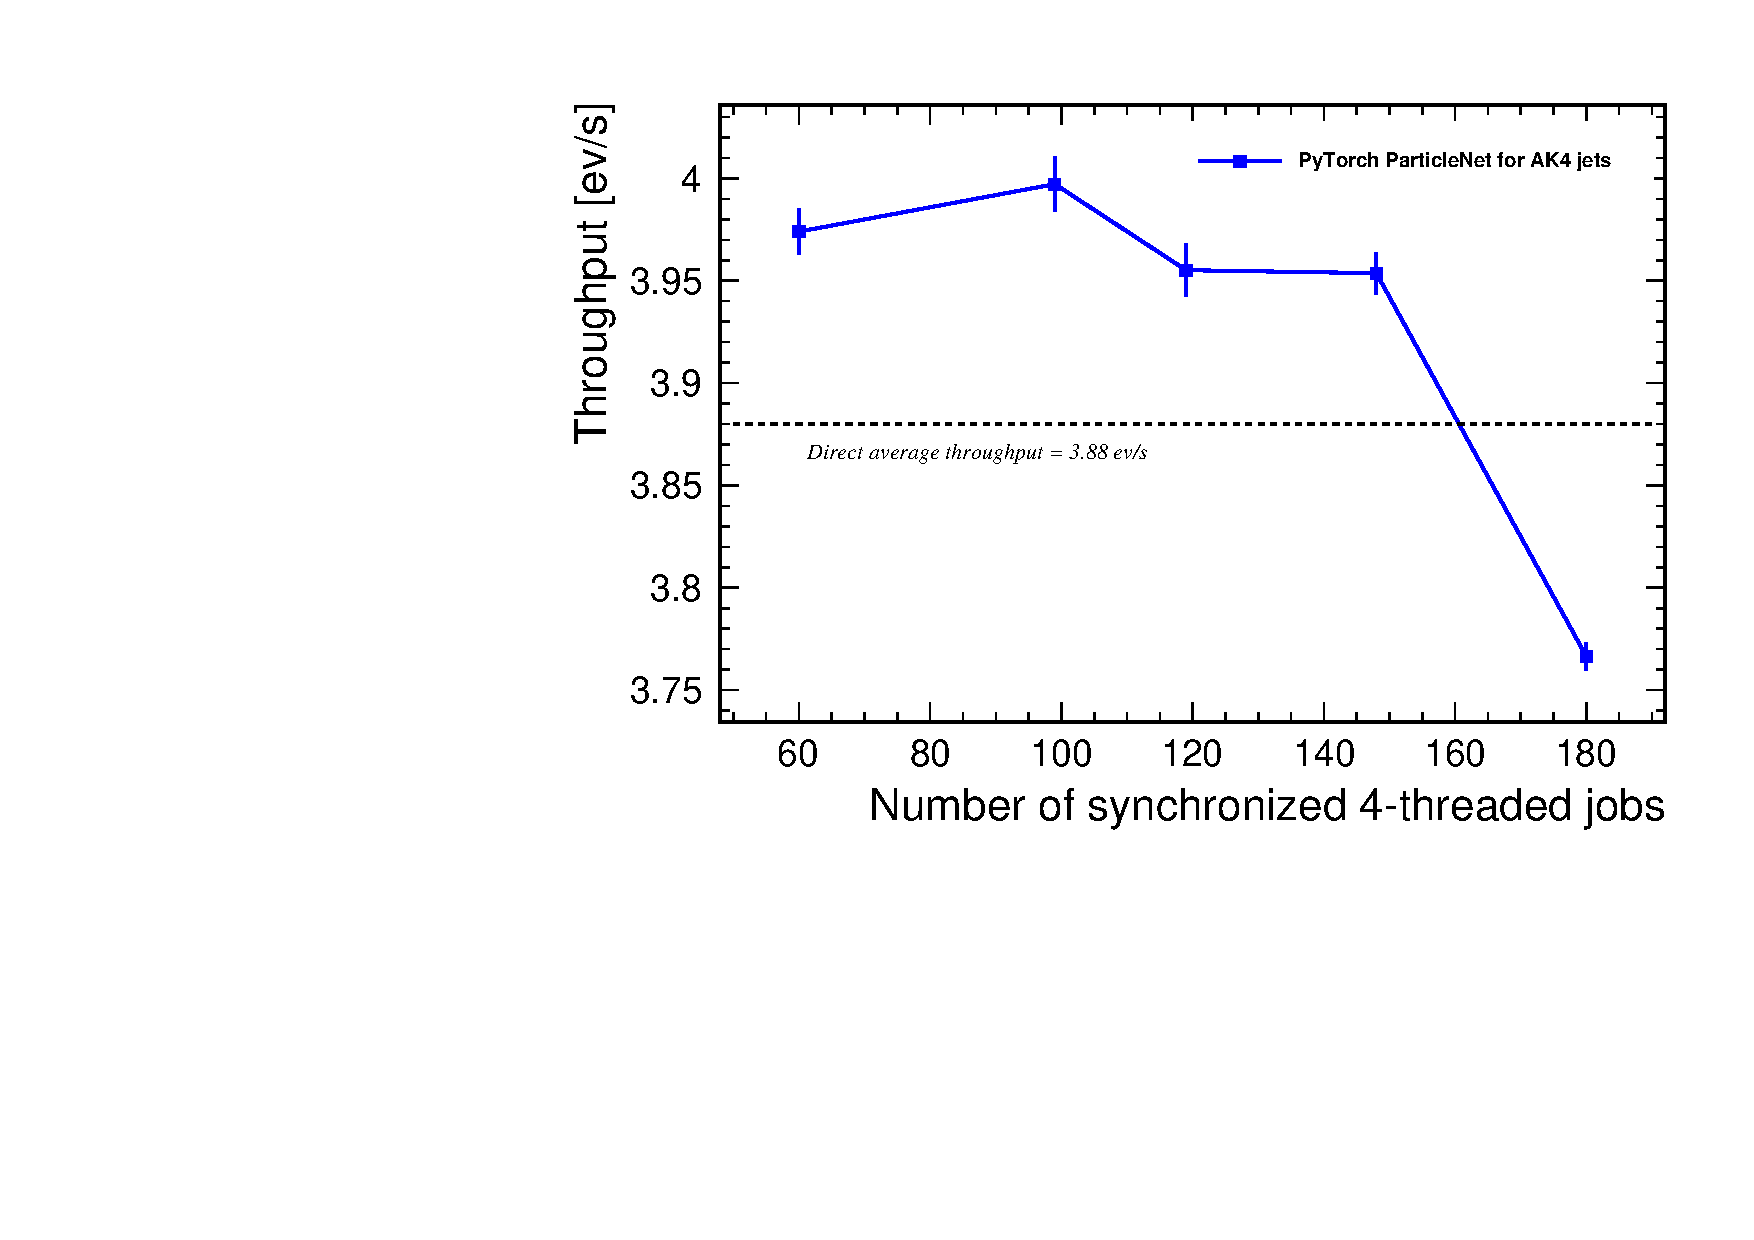
\includegraphics[width=0.70\textwidth]{plots/PN_throughput_scan_PT.pdf}
    \caption{GPU saturation scan performed in GCP, where per-event throughput is shown shown as a function of the number of parallel CPU clients for the \PYTORCH version of ParticleNet for AK4 jets (black), DeepMET (blue), DeepTau optimized with TRT (red), and all \PYTORCH versions of ParticleNet for AK8 jets on a single GPU (green). Each of the parallel jobs was run in a 4-threaded configuration.}
    \label{fig:throughputs_scan_pn}
\end{figure}

Similar analysis was performed for the other models. When all three flavors of PN for AK8 jets are hosted on a single GPU, that GPU can service about 195 simultaneous 4-threaded client jobs. For DT and DM, a single GPU hosting only one of the algorithms could service about 64 and 520 client jobs, respectively. The differences between these saturation points are mostly due to different model sizes and different number of objects per event. From these saturation values, it is possible to determine the number of GPUs that would be needed to service a production job that uses a large number of client side CPUs, and it is possible to determine the ratio of the number of GPUs hosting different models. For PN and DT, the saturation points will depend on the number of jets and taus in the events in the sample being processed, such that the ratio of GPUs hosting different models and the required ratio of GPUs to CPUs is sample-dependent. As long as dynamic batching is enabled, the number of GPUs required for a model will depend roughly linearly with the number of objects per event that require an inference; for example, if a sample had half as many jets per event, it would require roughly half as many GPUs to service PN, while the number of GPUs required for DM should not change, as that model makes one inference for all events.

It should also be noted that a single GPU can host multiple models. In practice, it was found that putting only a single model on each GPU led to about 3--5\% faster performance than putting every model on each GPU, and this split-model configuration was used in subsequent studies. However, in a scenario where samples with diverse physics content are being processing, using the every-model configuration could prove to be the most straightfoward option, though preparatory model profiling should still be performed to ensure that enough GPUs and model instances will be available.

\subsection{Cross-site tests}
\label{sec:different_sites}

At this point, it is worth addressing a potential bottleneck in the SONIC paradigm: increased inference latency due to physical distance between client and server and the network loads. While a previous study observed that the per-event latency difference between remote and on-premises servers is negligible~\cite{Krupa:2020bwg}, we tested this observation explicitly with the Mini-AOD workflow, with results presented in Fig.~\ref{fig:crosssites}. In this test, client-side jobs were executed at Purdue's Tier-2 computing cluster in Indiana. All the models are loaded into one server running on one single GPU for simplicity. The blue points and lines show the throughput improvement in the Mini-AOD workflow when the client jobs communicate with Triton servers hosting all models at the same time, running on a single GPU \textit{also physically located at Purdue}. The improvement is shown as a function of the number of synchronized 4-threaded client-side jobs running at once. It can be seen that the single GPU server begins to saturate when about 10 client side jobs are sending requests at once and that the SONIC-enabled Mini-AOD workflow becomes \textit{slower} than the CPU-only workflow if more than about 17 4-threaded client-side jobs are running at once.

The green points and line in Fig.~\ref{fig:crosssites} show the throughput improvement when the client side jobs are once again run at Purdue, while the Triton server hosting all models on a single GPU is run on GCP resources, which were \textit{physically located in Iowa} for this test. Both the observed throughput increase and observed GPU saturation point are about the same for both server locations, so we can safely conclude that server location has little impact on performance, at least for client-server separations on the order of hundreds of kilometers.

%To study the possible effects of data transfers between servers and clients, we test the performances of running GPU servers on different sites. Fig~\ref{fig:crosssites} shows the test results. The CMSSW CPU clients always run at Purdue, while the servers run at Purdue and Cloud. The improvements are both around 10\% compared with directly-connected case, and the saturation point are very close. So we conclude with the current setup there is no significant impacts when running servers at different sites.

\begin{figure}[htp]
    \centering
    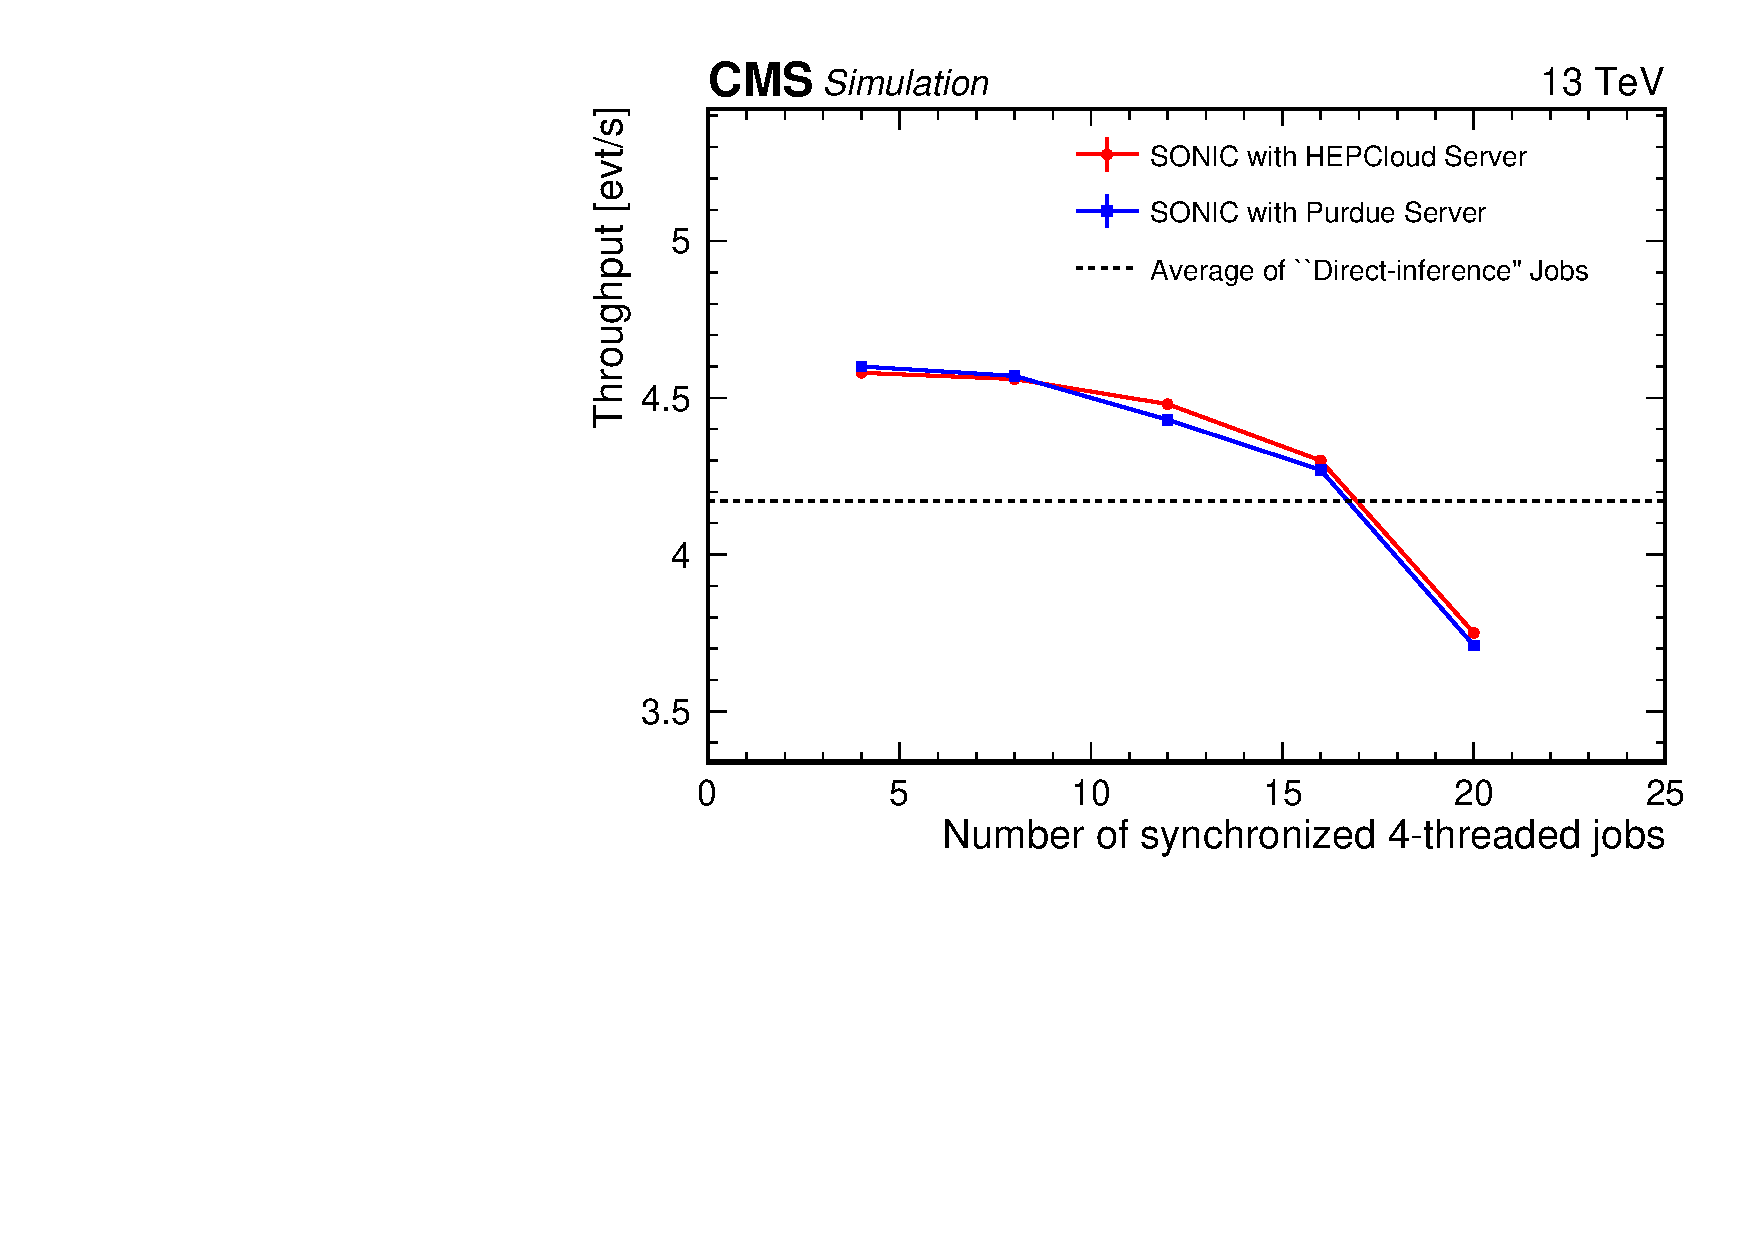
\includegraphics[width=0.60\textwidth]{plots/throughput_crosssite.pdf}
    \caption{Production tests across different sites. The CPU tasks run at Purdue, while the servers with GPU inference tasks run at Purdue (Blue) and Cloud (Red).}
    \label{fig:crosssites}
\end{figure}

\subsection{Large-scale tests}
\label{sec:scale_out}

Finally, we run tests performed at large scale, meant to emulate realistic Mini-AOD production scenarios. This test was performed exclusively in GCP. Here, 24 NVIDIA Tesla T4 GPUs were used to host the PT version of PN for AK4 jets, 20 GPUs were used to host the PT version of all three PN models for AK8 jets, 48 GPUs were used to host DT, and 10 GPUs were used to host DM. The ratios of the number of GPUs hosting each model may not exactly match that expected from Section~\ref{sec:different_sites}; this was done because the input/output bandwidth for VMs in GCP is restricted for virtual machines with fewer CPU-cores. To maximize the allowed bandwidth, it was easiest to start up virtual machines with 4 GPUs, which is why the numbers of GPUs used for most models come in multiples of 4. For DM, two 4-GPU VMs were used along with one 2-GPU machine. Clients accessed these virtual machines via a Kubernetes load-balancer, which provided a single IP address for each model type and distributed inference requests evenly among the servers.

Client-side jobs also ran on CPU-only GCP resources, using HepCloud to dynamically allocate preemptible resources and assign jobs to the client-side VMs. Each client job was run in a 4-threaded configuration, with input data files stored locally, and each VM created in this HepCloud setup had 32 cores and 163\,840\unit{MB} of memory, meaning up to 8 simultaneous jobs could run in a single VM.

The largest test had 2\,500 synchronized client-side jobs, which amounts to 10\,000 CPU-cores. Because these jobs were run on preemptible resources, Google reserves the right to re-allocate any VM to higher priority requests from other GCP users. Of the 2\,500 job, 2\,455 completed successfully without preemption, so in the end 9\,820 client-side CPUs were used.

Preemptible resources were used to reduce the costs of running single tests. Similarly, we used a larger number of GPUs than strictly necessary to avoid the possibility that performance would \textit{not} meet the expectations from the tests described in Section~\ref{sec:algo_acceleration}, and thereby to avoid the cost of having to repeat the test potentially multiple times. For instance, based on a single-GPU saturation point of 115 4-threaded jobs, one would expect that only about 22 GPUs would be needed to service the AK4 jet PN model. So while the demonstration illustrated here uses a CPU:GPU ratio of 96:1, achieving a higher ratio is very likely possible.

The results of this large-scale test are shown in Fig.~\ref{fig:scaleout}. The SONIC-enabled jobs achieved an average throughput of 4.01 events per second, while CPU-only benchmarking jobs had a throughput of 3.55 events per second. This 12\% speed-up in throughput is about what would be expected from removing the PN, DT, and DM inference from the total MiniAOD latency.

\begin{sloppypar}As mentioned before, server-side VMs were optimized to allow maximal input and output bandwidth. No bottlenecks due to bandwidth were observed in this scale-out test. We noted that the maximum rate of bytes received by one of the Kubernetes load-balancers was 11.5\unit{GB/s}, which was for DT. The next-highest data input rate was 3.3\unit{GB/s} for DM, and less than 500\unit{MB/s} of input was needed for all PN models combined. The output rate was significantly smaller for each model, as most return only one or a few floating-point values as the inference result.\end{sloppypar}

%discuss server-side CPU requirements?

%We perform the scale-out tests at GCP. We run around 2500 CMSSW jobs on 10K CPU cores at GCP, each job with 4 threads. The three algorithms are offloaded to around 100 NVIDIA T4 GPUs. The jobs run well with no significant issues. Fig~\ref{fig:scaleout} shows the throughput distributions of these CMSSW jobs. Compared with the directly-connected case running on CPUs (orange), we observe about 12\% throughput improvements, as expected.

\begin{figure}[htp]
    \centering
    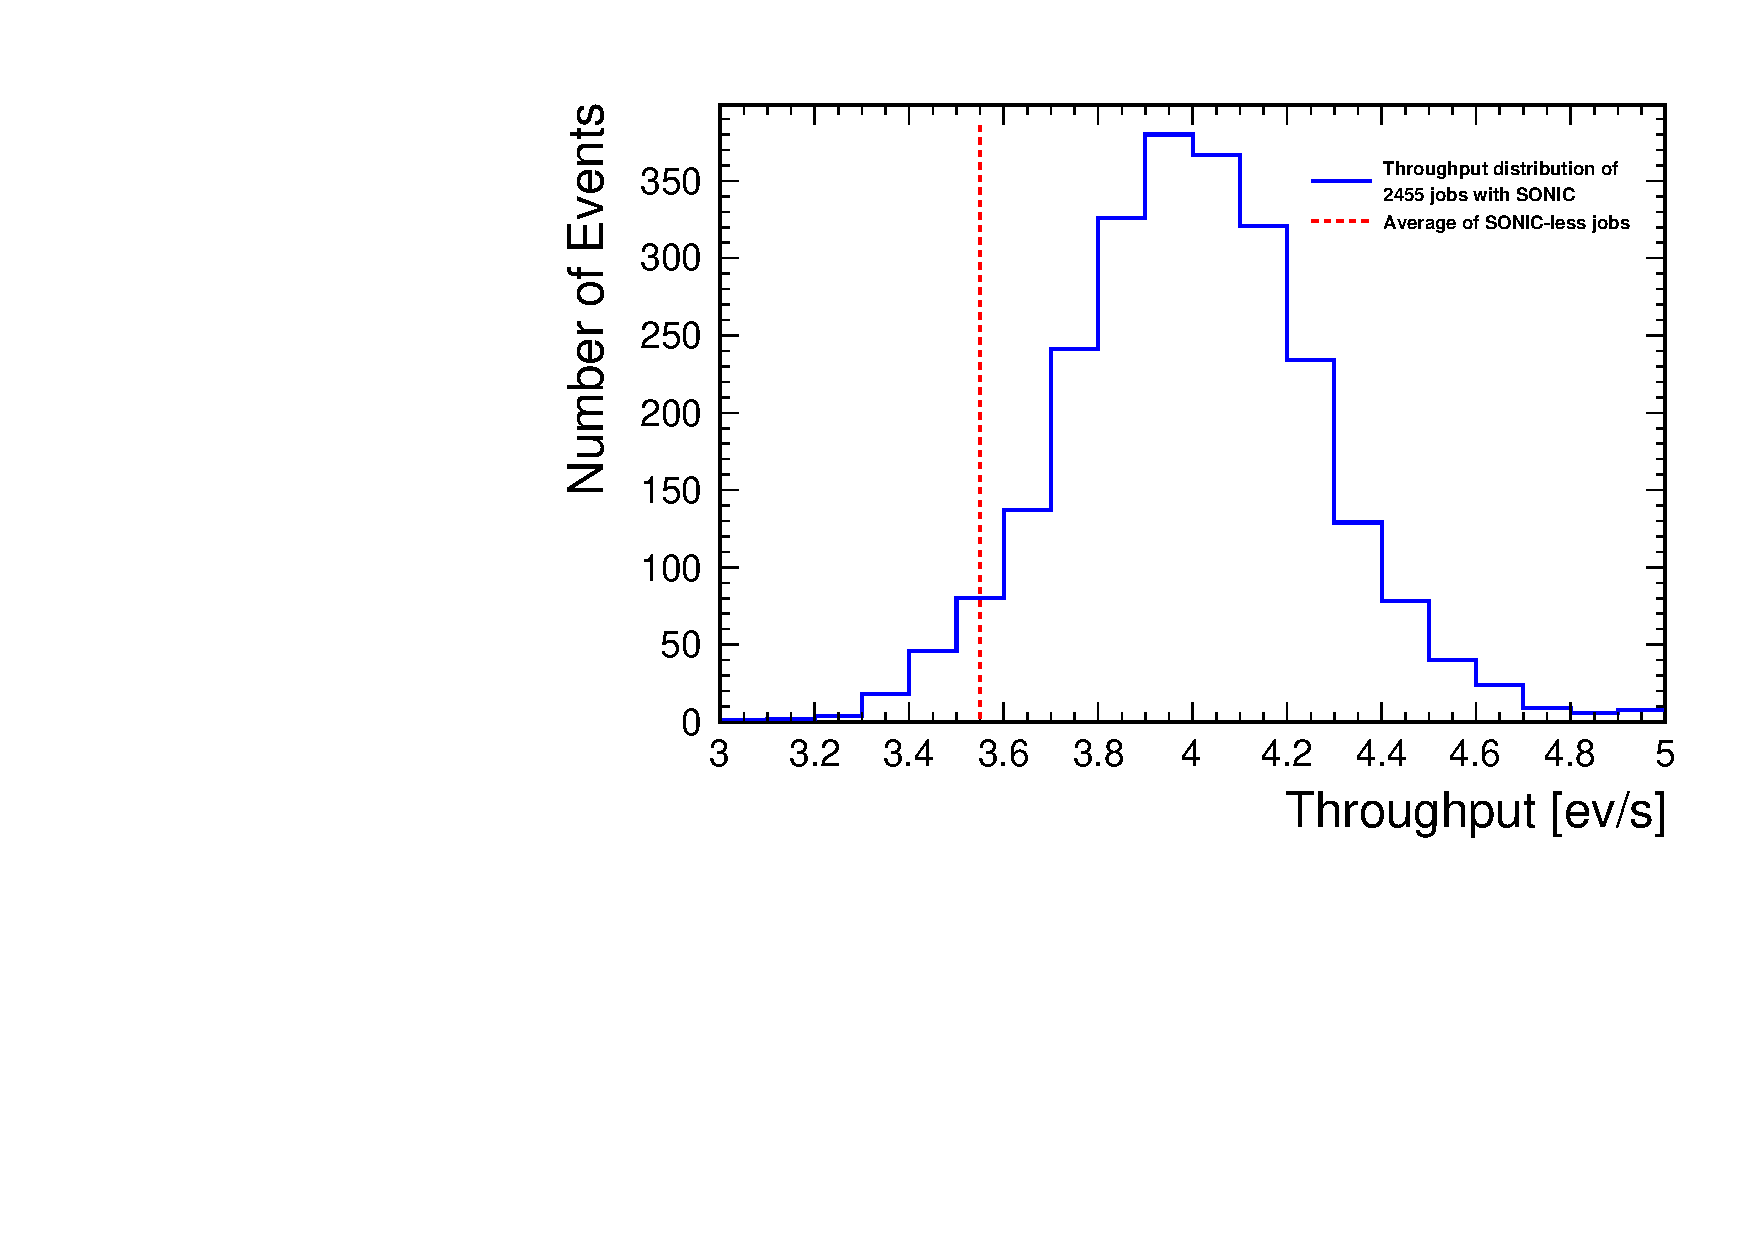
\includegraphics[width=0.70\textwidth]{plots/scale_out_test_reformat.pdf}
    \caption{Scale-out test results at Google Cloud. The average throughput of the SONIC-enabled workflow was 4.01\unit{evt/s}, while the average throughput of the ``direct-inference" workflow is 3.55\unit{evt/s} (dashed red) with a variance of around 2\%. The SONIC-enabled workflow thus achieves a throughput that is 12\% faster than the CPU-only version of the workflow.}
    \label{fig:scaleout}
\end{figure}



\section{Portability}
\label{sec:IPUs}
While the inference servers discussed so far have exclusively utilized GPU resources, servers are easily portable and can run on other processing platforms. In particular, we have studied running the Mini-AOD workflow with servers on CPUs and Graphcore Intelligence Processing Units (IPUs)~\cite{Graphcore}.

\subsection{CPU fallback server}
\label{sec:fallback}
%As discussed in Section~\ref{sec:sonic_benefits}, SONIC can factorize the ML software frameworks out of the client. Therefore, SONIC can be used as the default approach for inference even on local CPUs, eliminating the need to integrate third-party direct ML inference framework support into the experiment software (CMSSW). In addition, w
When running with remote servers, one potentially common and important failure mode is communication errors between clients and servers. In order to support automatic local CPU inference as a backup option when communication failures occur with remote servers, the SONIC implementation includes a service that can launch a Triton server using local CPU resources for any SONIC-compatible models, referred to as a ``fallback server''. Fallback servers can also be used for inferences when third-party ML frameworks are not supported yet for direct inferences. 

Ideally, the use of fallback servers should have minimal impact on per-event throughput relative to running direct-inference jobs without SONIC. This is contingent on two factors. Firstly, the latency introduced by sending data to/from local servers must be negligible. Secondly, servers should introduce minimal overhead in order to consume as few CPU resources as possible beyond what is needed to perform inference. The first concern can be resolved using the shared-memory option, which skips the gRPC communications and directly pass between servers and clients the data in a certain memory chunk. In reality, the gRPC overhead in most cases is found to be negligible. For the second concern, since local servers are running on the same CPUs as the other modules in the workflow, scheduling should be placed to avoid CPU thread contention between the two. This implies synchronous mode is preferred for local CPU fallback servers. Inference tasks should not create extra threads to avoid contentions. In the experiments we have found that more inference threads than the CMSSW job threads will slow processings down dramatically.

After some explorations, for the local CPU inferences we decide to choose to run in synchronous mode, with the number of model instances set to the number of threads per job, and number of inference thread always 1. This way it can mimic the direct inference and avoid thread over-subscriptions as much as possible. We compare the throughputs between direct inferences and SONIC with local CPU servers with such configurations. Tests were performed using resources at the Purdue Tier-2 cluster with the CPU-only nodes. There are $n_{\text{CPU}}=20$ Intel E5-2660 CPU cores on one node, and hyperthreading is disabled to ensure more stable results. For all tests, the CPU nodes are always saturated by having the product of the number of jobs ($n_j$) and number of threads per job ($n_T$) to be the number of CPU cores: $n_j\times n_T = n_{\text{CPU}} = 20$. We scan the throughput as a function of the number of threads, as shown in Fig.~\ref{fig:throughput_cpu}. After optimizations, the throughputs of running on the local CPU fallback server are very similar to direct inference now. The higher throughputs in some cases are due to more recent versions of ONNX inference version installed inside the server, which can be controlled in the real productions.

\begin{figure}
    \centering
    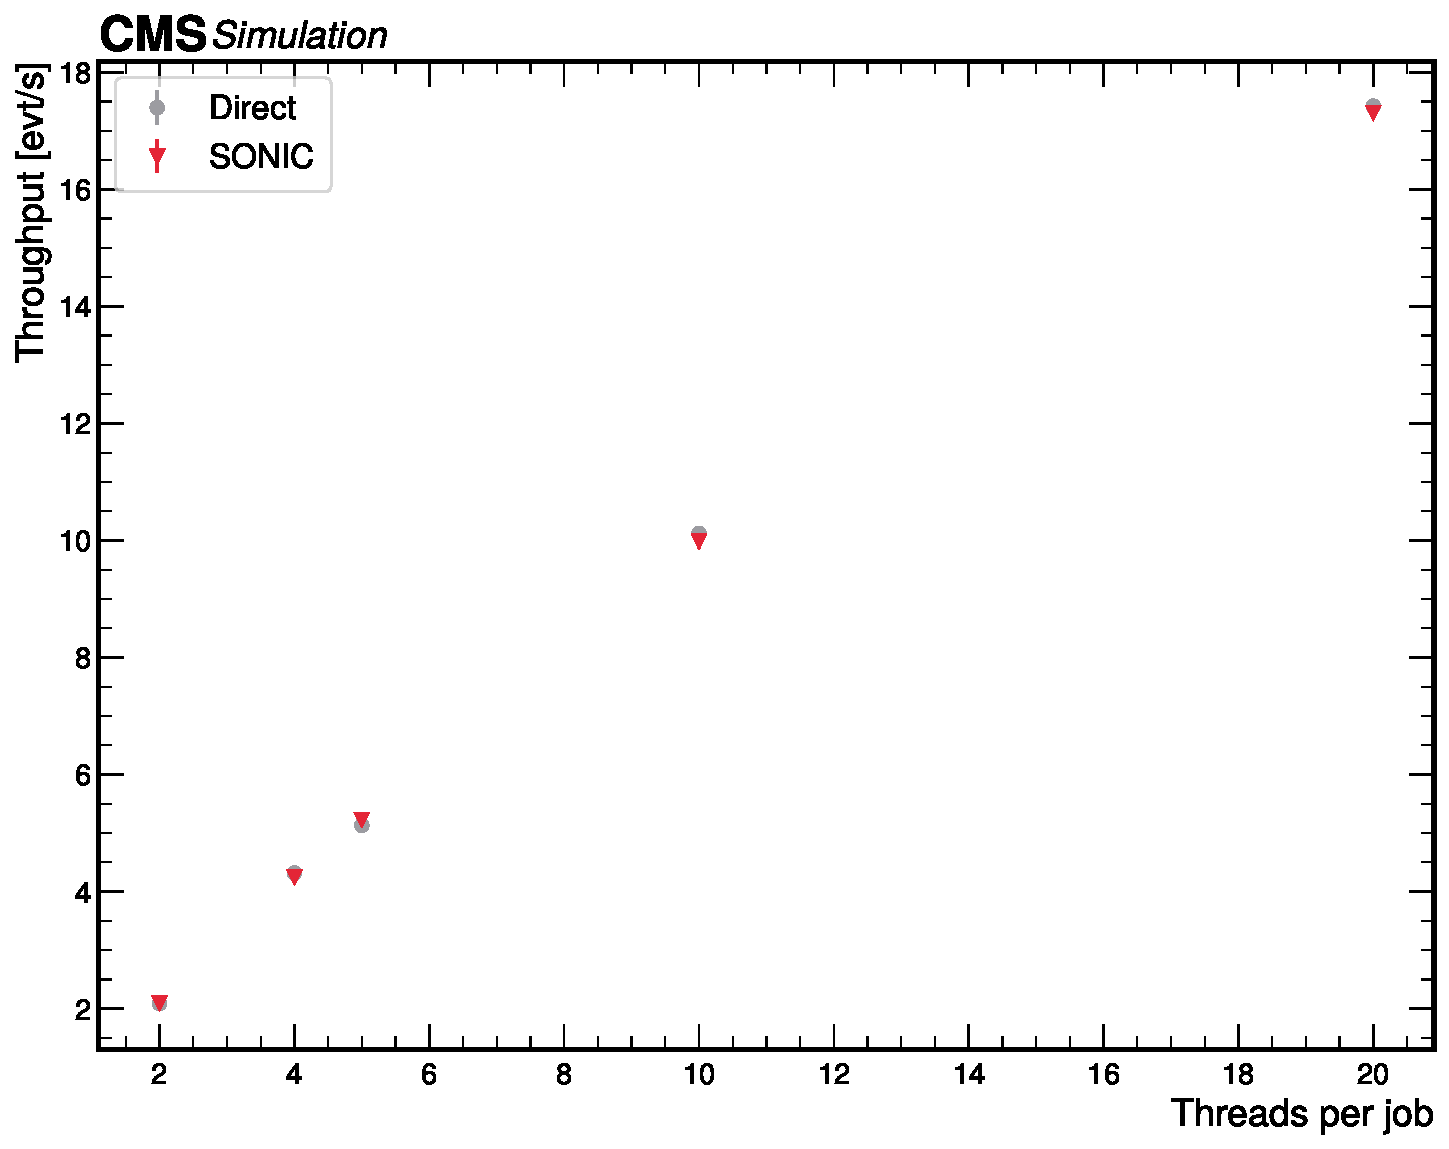
\includegraphics[width=0.48\textwidth]{plots/threads_vs_throughput.pdf}
    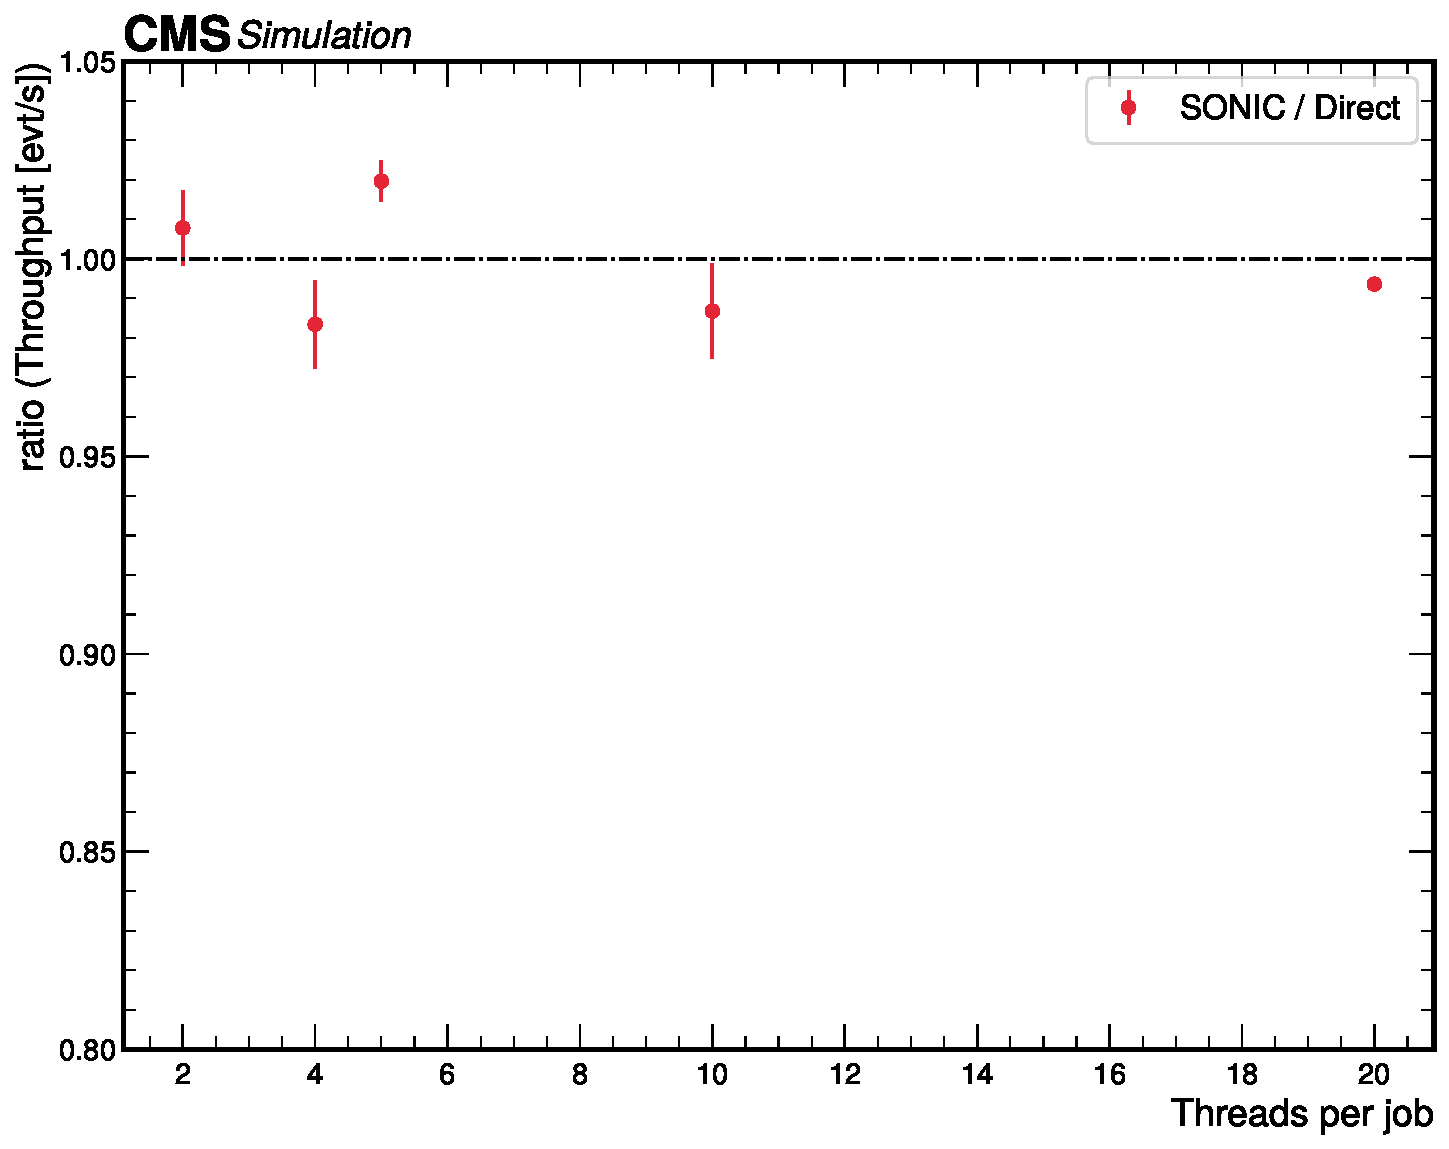
\includegraphics[width=0.48\textwidth]{plots/threads_vs_throughput__ratio.pdf}
    \caption{Throughput (left) and throughput ratios (right) of different configurations of the CPU saturation tests at Purdue Tier-2 Cluster.}
    \label{fig:throughput_cpu}
\end{figure}


\subsection{Studies with Graphcore IPUs}
\textcolor{red}{Detailed contents are still under discussion with GraphCore team.}

As discussed in Sections~\ref{sec:triton} and~\ref{sec:sonic_benefits}, NVIDIA Triton inference servers support custom backends to run with different coprocessors and different (ML) backends. Since the SONIC client code only depends on the Triton protocols, algorithms implemented in this way can easily be ported to different types of coprocessors. One of the Mini-AOD production tests was done together with the GraphCore IPU team, where they prepared a custom backend to support running ML inference with IPUs. The current supported ML frameworks include \TENSORFLOW and \PYTORCH, with \ONNX and \PYTORCHGEOMETRIC support in development. This allows us to run DeepMET and DeepTauID inference on IPUs. Without any modifications on the client side, we reconfigure the workflow configuration to point the clients to IPU servers on the Graphcloud cluster, and successfully run DeepMET and DeepTauID models via SONIC, while running the other parts of the Mini-AOD workflow on local CPUs.


\section{Summary}
\label{sec:summary}
Within the next decade, the data taking rate at the LHC will increase dramatically, straining the expected computing resources of the experiments running on it. At the same time, more and more of the algorithms that will be run on these resources are being converted into either ML or domain algorithms that are easily accelerated with the use of coprocessors, such as GPUs. Therefore, by pursuing heterogeneous architectures, it is possible to alleviate potential shortcomings of available CPU resources.

IaaS is a promising scheme to integrate coprocessors into CMS computing workflows. In IaaS, client code simply assembles the input data for an algorithm, sends that input to an inference server running either locally or remotely, and retrieves output from the server. The implementation of IaaS discussed throughout this paper is called SONIC. SONIC employs NVIDIA Triton Inference Servers to host models on coprocessors, as demonstrated here in studies on GPUs, CPUs, and IPUs. %In general, using SONIC in CMSSW has many benefits relative to writing a custom mechanism for interacting with coprocessors: it factorizes ML frameworks out of CMSSW, allowing for more diverse algorithms; it simplifies client code, which only needs to send data to the server and retrieve output; it enables more efficient use of resources, as the coprocessor to CPU ratio can be tuned; client code does not need to be adjusted to use different types of coprocessors for inference acceleration; and it is the only way to use remote coprocessor resources.

In this paper, the use of SONIC in CMSSW is demonstrated in a sample Mini-AOD workflow, where a jet tagging algorithm, a tau identification algorithm, and a missing transverse energy regression algorithm are ported to inference servers. These algorithms account for 10\% of per-event latency in a sample of Run 2 \ttbar events. After a demonstration of model-profiling, which is used to optimize server performance and determine the needed number of GPUs for a given number of client jobs, we showed that the expected 10\% decrease in per-event latency was achieved in a large scale test of SONIC-enabled Mini-AOD production that used about 10\,000 CPU cores and 100 GPUs.

In addition to meeting performance expectations, we demonstrated that the per-event latency is not highly sensitive to physical client-to-server distance, and that running inference through Triton servers on local CPU resources does not increase latency relative to the standard approach of running inference directly on CPUs in the job thread. We were also able to perform a test of SONIC on GraphCore IPUs to demonstrate the flexibility of our approach.

The SONIC approach for IaaS represents a flexible approach to accelerate algorithms, which is increasingly valuable for LHC experiments. Using a realistic workflow, we have highlighted many of SONIC's benefits, which we believe make it a leading paradigm for the future of CMS computing.

%In this paper we have presented the studies of running inference as-a-Service via SONIC, with the CMS Mini-AOD production workflow as the motivating case. The benefits of running SONIC are discussed, and the studies of running different models with different ML backends are compared. We have observed the expected gains by offloading ML inferences to (remote) GPUs via SONIC, with negligible overhead for servers running at different sites. The whole framework can run also on different types of coprocessors such as IPUs, and scales up well for large-scale productions. Studies are also done for optimizing inference performances on local CPUs. 

%With more and more ML algorithms being developed and integrated into the production workflow, these studies are becoming more and more interesting and important to provide an approach for solving the computing challenge.


\clearpage
% Correct ones will be incerted later
\begin{acknowledgments}
\end{acknowledgments}

\bibliography{ML-23-YYY}
